\appendix
\section{Extended numerical verification and comparison}\label{app:numerics}

This appendix collects the full figure-by-figure evidence summarised in
Section~\ref{sec:results}: the per-result verification maps, the simulation cross-checks, the
extended traffic-intensity and mechanism sweeps, the class-asymmetry study, the convergence
diagnostics, and the synoptic dashboard. Unless stated otherwise all figures use the base
parameters of Section~\ref{sec:results} --- $\lambda_1=0.3$, $\lambda_2=0.4$, $\mu=1.0$, with
the mechanism parameter ($\gamma_1$ or $\theta_1$) set to $0.5$ where applicable --- and the
truncated CTMC ($N_{\max}=40$) as ground truth.

% =====================================================================
\subsection{Verification against the CTMC}\label{app:numerics:validation}

These figures provide the visual evidence behind the verdicts of
Table~\ref{tab:validation_summary}.

\subsubsection*{Structural lemmas}

The lemmas assert that the stationary distribution satisfies a specific
functional equation, so a non-vanishing residual would indicate either a
derivation error in the lemma or a coding error in the solver.
Figure~\ref{fig:val_lemmas} shows the maximum relative residual
$|{\rm LHS}-{\rm RHS}|/|{\rm RHS}|$ of each lemma's functional equation,
evaluated on the exact CTMC distribution across all model variants.
Both lemmas hold to better than $10^{-9}$ --- consistent with truncation noise at
$N_{\max}=40$, not formula error --- and Lemma~\ref{lem:gen:PPGF_dynamics} reaches floating-point
precision (${\sim}10^{-15}$) because its recurrence involves only one
discrete variable.

\begin{figure}[H]
    \centering
    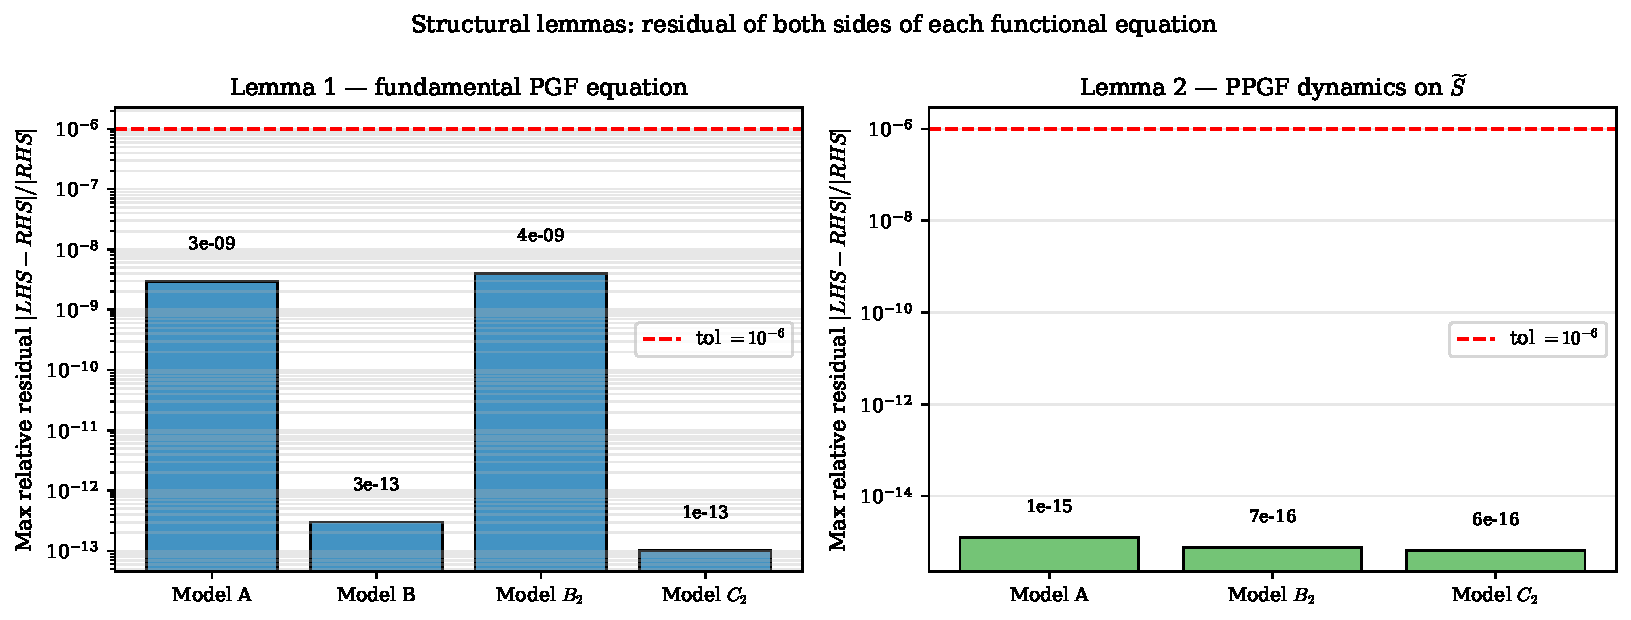
\includegraphics[width=0.90\textwidth]{figures/validation/val_lemmas.pdf}
    \caption{Lemma verification.  \textit{Left}: max relative residual of the
    fundamental PGF equation (Lemma~\ref{lem:gen:fundamental_equation}) for
    each model variant on a $5\times5$ interior grid.
    \textit{Right}: max relative residual of the PPGF dynamics recurrence
    (Lemma~\ref{lem:gen:PPGF_dynamics}) over $n\in\{1,\ldots,15\}$ and
    $y\in[0.05,0.90]$.
    All values lie well below the $10^{-6}$ tolerance (red dashed line).}
    \label{fig:val_lemmas}
\end{figure}

\subsubsection*{Closed-form and integral-form theorems}

Figures~\ref{fig:val_pxy} and~\ref{fig:val_py} compare the three analytic
formulas against the CTMC on a uniform grid, using identical parameters and
the same error metric; since only the extra mechanism changes between panels,
the errors are directly comparable. Model-$C_2$ reaches near-machine precision
because its closed form evaluates exactly through the Pollaczek--Khinchine
ratio; Model-$B_2$'s accuracy (${\sim}10^{-7}$) is limited instead by the
numerical quadrature of its integral representation, whose integrand steepens
near the branch point at $x=y$.

\begin{figure}[H]
    \centering
    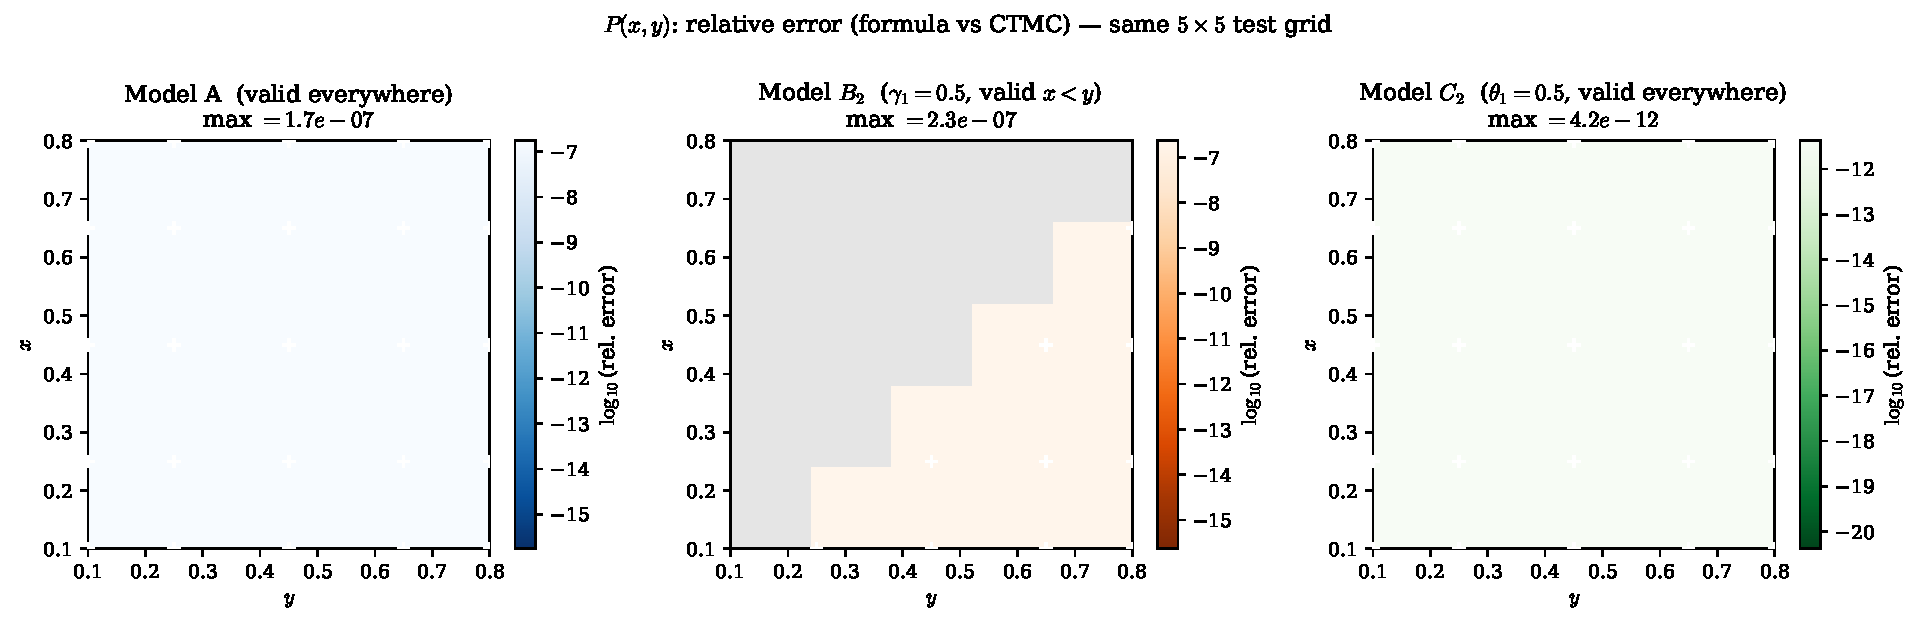
\includegraphics[width=\textwidth]{figures/validation/val_theorems_pxy.pdf}
    \caption{Relative error $|P_{\rm formula}(x,y)-P_{\rm CTMC}(x,y)|/|P_{\rm CTMC}(x,y)|$
    on the same $5\times5$ test grid for Models $A$, B$_2$, and C$_2$.
    Colour scales are anchored to the same range across all three panels.
    White crosses mark the 25 test points.}
    \label{fig:val_pxy}
\end{figure}

\begin{figure}[H]
    \centering
    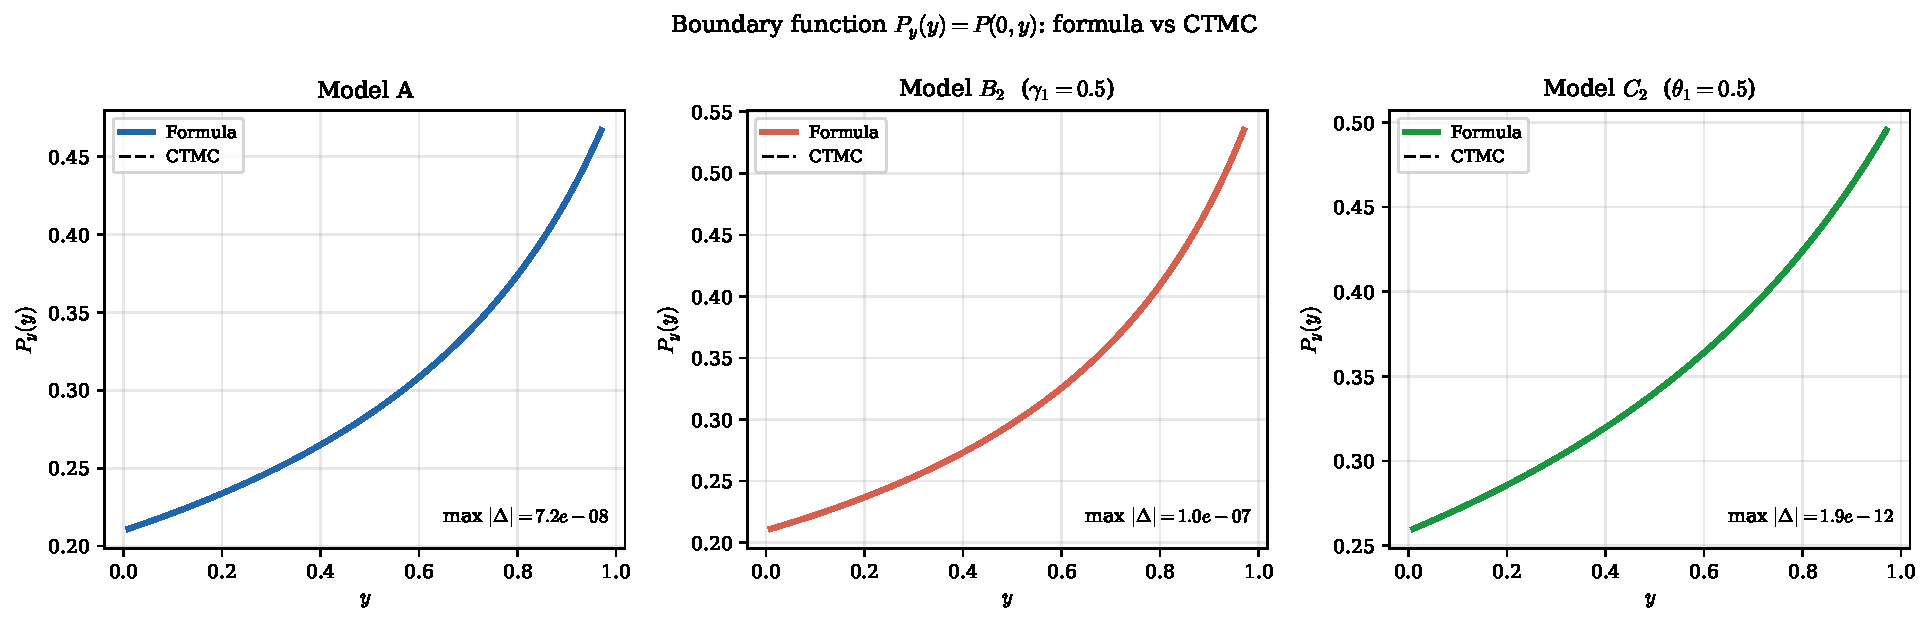
\includegraphics[width=\textwidth]{figures/validation/val_theorems_py.pdf}
    \caption{Boundary function $P_y(y)=P(0,y)$ for Models $A$, B$_2$, and C$_2$:
    analytic formula (solid) vs CTMC (dashed). All three curves rise
    monotonically to $P(0,1)$, the probability that the server is busy with an
    empty priority queue, but their levels differ: each mechanism changes how
    class-1 customers block class-2 service.}
    \label{fig:val_py}
\end{figure}

\subsubsection*{Corollaries}

The two corollaries are structurally very different: for the conserving models
($A$, $B$, $B_2$) the empty-state probabilities depend on the parameters only
through the total load $\rho$, whereas the Model-$C_2$ expressions run through
the busy-period mean $\mathbb{E}[B_C]$ and hence the confluent hypergeometric
function. Both are tested identically.
Figure~\ref{fig:val_corollaries} shows the scatter of formula vs CTMC values
for $\pi_0$ and $\pi(0,0)$ across 60 random parameter configurations for each
corollary.  All points lie on the diagonal to within $10^{-4}$.

\begin{figure}[H]
    \centering
    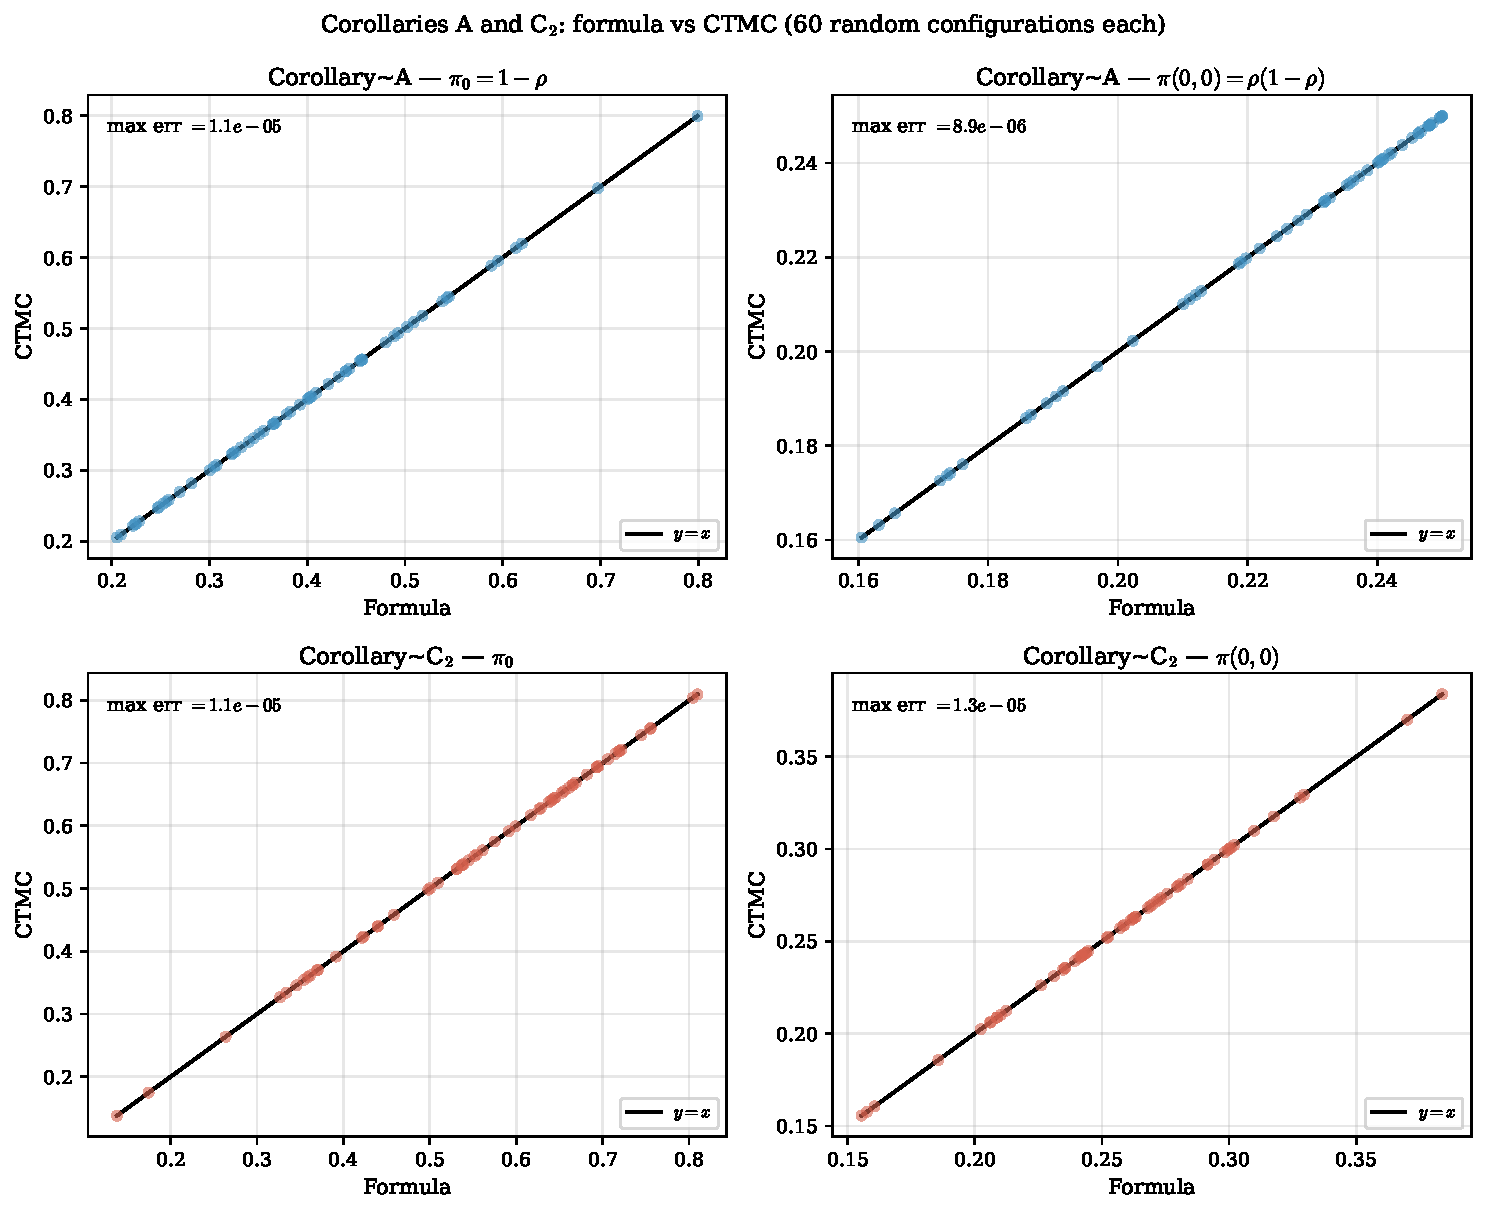
\includegraphics[width=0.80\textwidth]{figures/validation/val_corollaries.pdf}
    \caption{Corollaries A (blue) and C$_2$ (red): formula vs CTMC for
    $\pi_0$ (left column) and $\pi(0,0)$ (right column) over 60 random
    configurations each.  Perfect agreement lies on the diagonal. The C$_2$
    corollary, despite running through the $M/M/1+M$ busy period and the
    confluent hypergeometric function, matches the CTMC to the same tolerance
    as the rational Model-$A$ formula.}
    \label{fig:val_corollaries}
\end{figure}

\subsubsection*{PPGF approximation (Approximation~\ref{apx:A:PPGF_Stilde})}

Unlike the exact results of Table~\ref{tab:validation_summary}, this result is
approximate by design: the recursion drops the boundary-diagonal forcing term,
which decays geometrically in $n$, so the approximation is exact at $y=1$ for
all parameters but degrades wherever the neglected forcing competes with the
homogeneous solution. Figure~\ref{fig:val_ppgf} maps the maximum relative error
$\varepsilon_\infty(\rho_1,\rho_2)$ over the parameter space and confirms the
validity region characterised in \S\ref{ssec:A:Stilde}: the priority-dominated,
moderately loaded regime. This is the single conditionally accepted result of the
verification exercise ---assessed separately from Table~\ref{tab:validation_summary}---
and the one place where the alternative coordinatisation
$\widetilde{S}$ does not yield an exact result.

\begin{figure}[H]
    \centering
    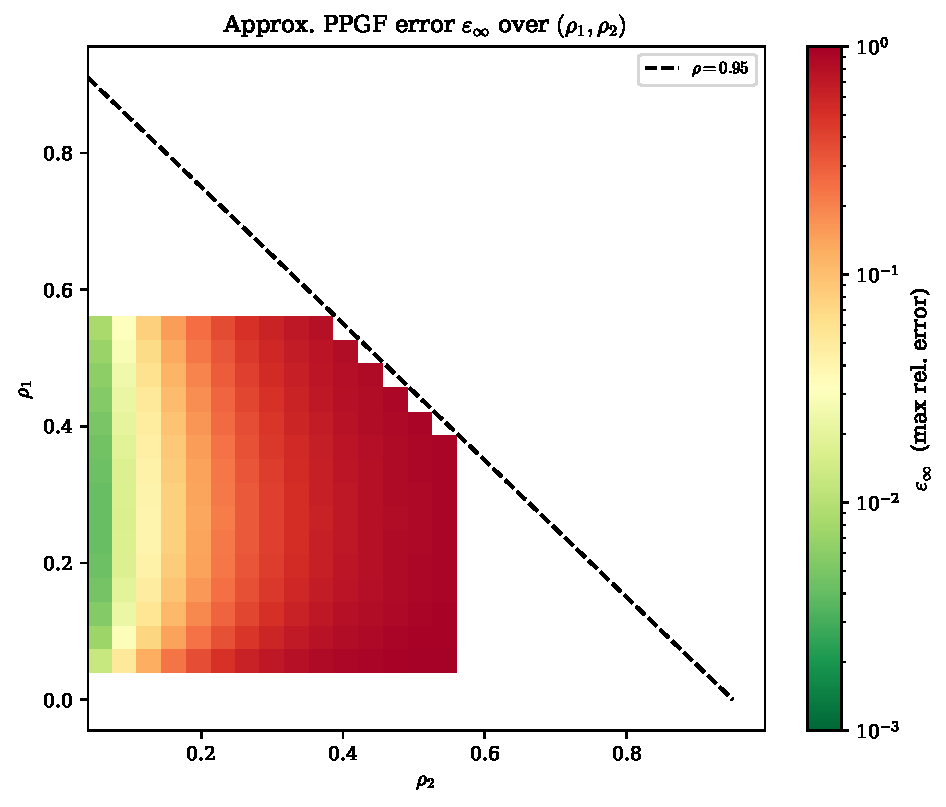
\includegraphics[width=0.52\textwidth]{figures/validation/val_ppgf_heatmap.pdf}
    \caption{Max relative error $\varepsilon_\infty$ of the approximate PPGF
    $\widetilde{P}_{\rm app}(y,n)=(1-\rho)\rho[\widetilde{y}^*(y)]^n$ as a
    function of $(\rho_1,\rho_2)$.
    \emph{Colour convention} (shared with the $\mathbb{E}[N_1]$ heatmap,
    Figure~\ref{fig:c2:heatmap}): \textcolor{green!60!black}{green} marks the
    accurate regime ($\varepsilon_\infty<3\%$) and \textcolor{red}{red} the
    inaccurate one---green favourable, red unfavourable, in the same direction
    across both maps.
    The approximation is reliable only when the priority class carries most
    of the offered load ($\rho_1/\rho\gtrsim0.6$) and the system is not
    heavily loaded ($\rho\lesssim0.6$).}
    \label{fig:val_ppgf}
\end{figure}

\subsubsection*{Head-of-line models \texorpdfstring{$\BH$}{B2-H} and \texorpdfstring{$\CH$}{C2-H}}

The two head-of-line models possess algebraic fundamental equations.  The lemma
check therefore requires no differentiation of $P$: only the CTMC values of
$P(x,y)$ and $P_y(y)$ are substituted into each side and the residual is
measured. The theorem check is the same $P(x,y)$ grid comparison used for
Models~$A$, $B_2$, and $C_2$. Figure~\ref{fig:val_experiment} reports both checks, and
Figure~\ref{fig:val_experiment_pi} tracks the empty-state probabilities $\pi_0$
and $\pi(0,0)$ as the mechanism parameter grows.

\begin{figure}[H]
    \centering
    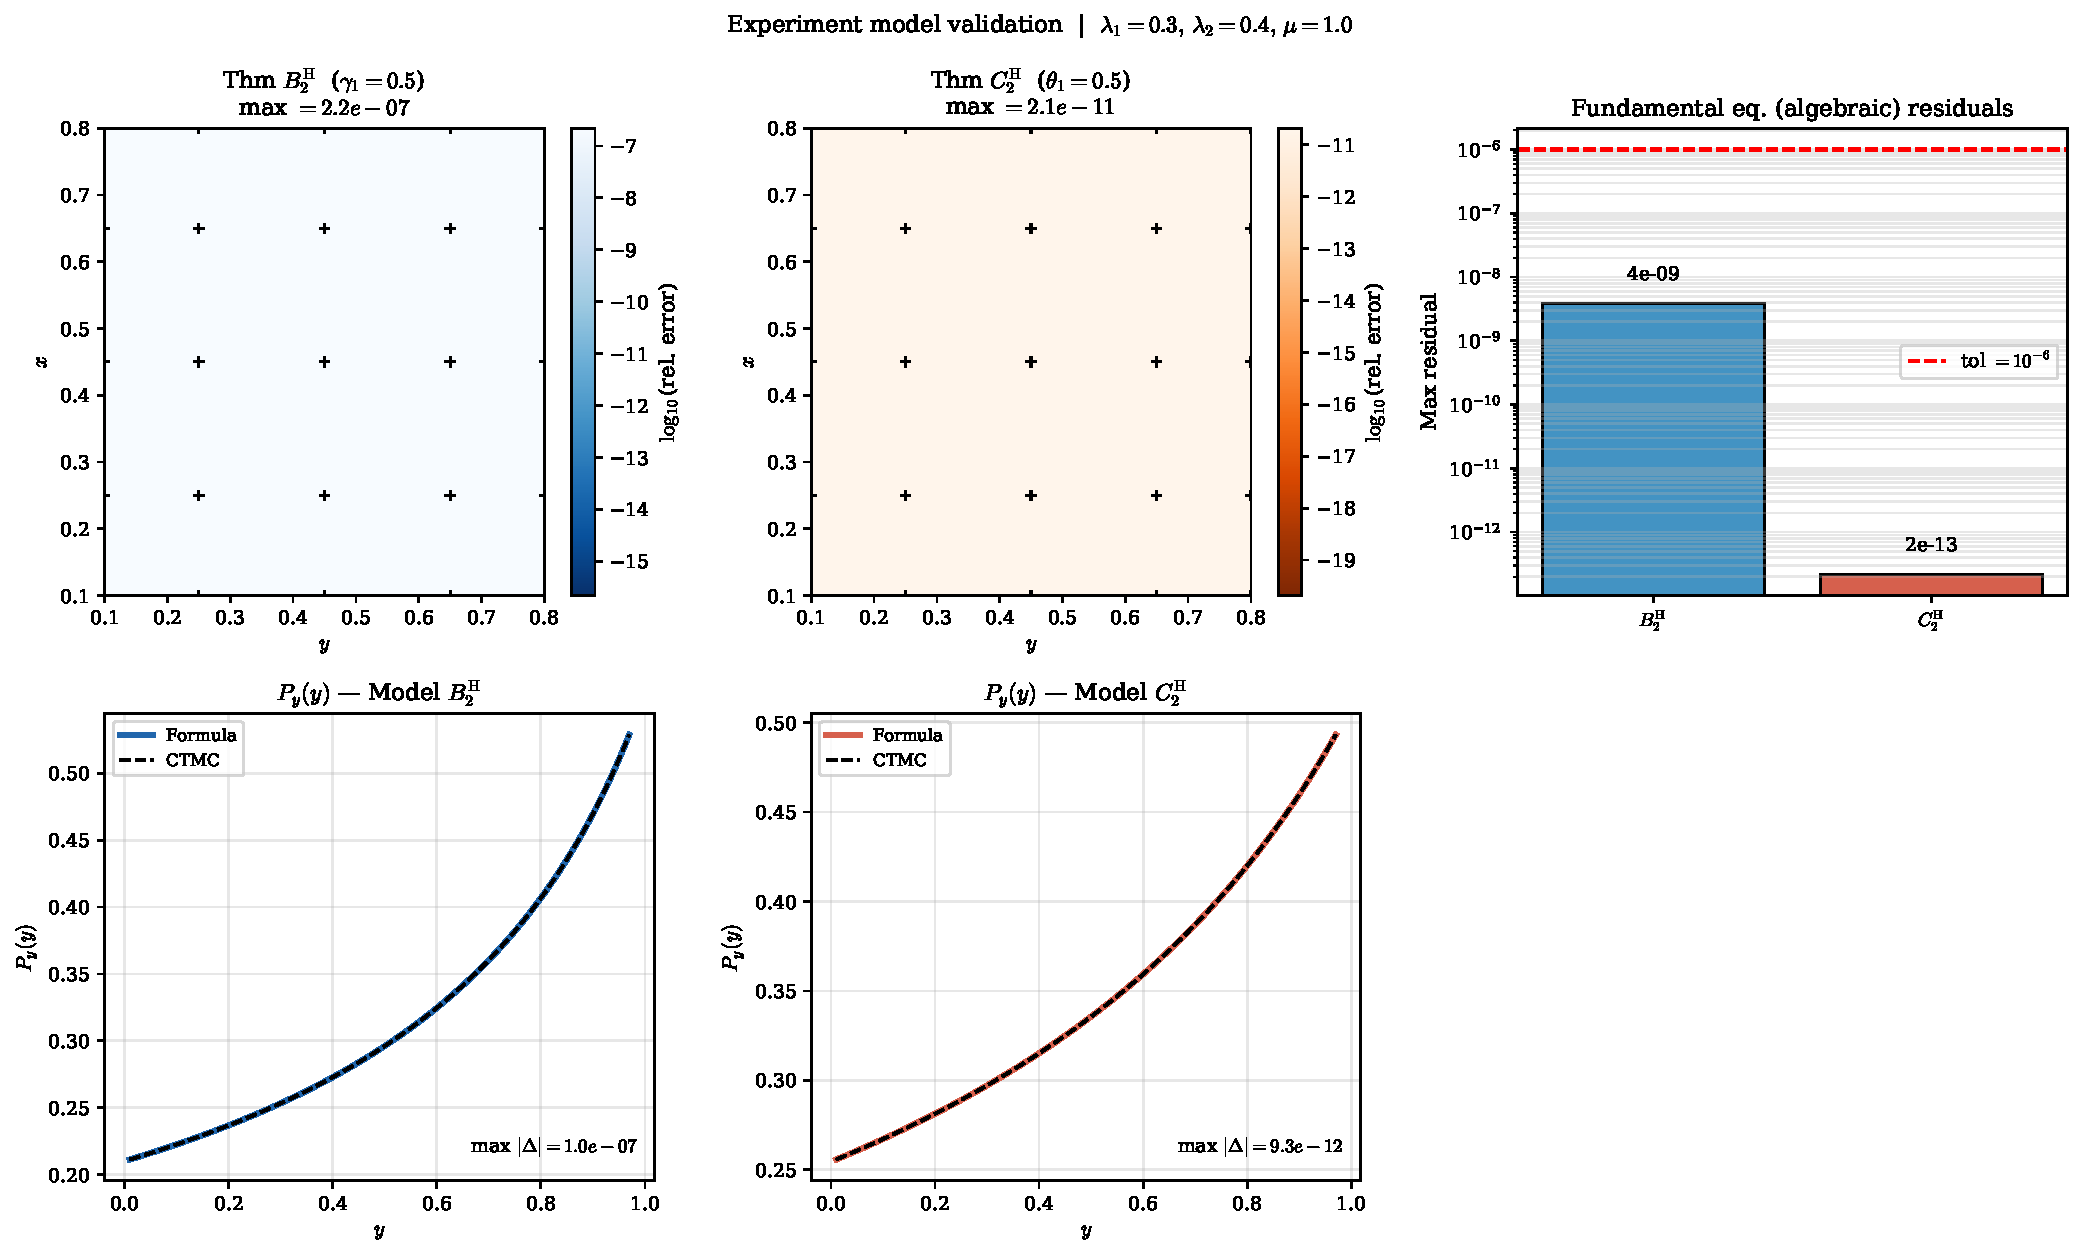
\includegraphics[width=\textwidth]{figures/validation/val_experiment.pdf}
    \caption{Verification of Models $\BH$ and $\CH$.
    \textit{Top row, left and centre}: relative error
    $|P_{\rm formula}(x,y)-P_{\rm CTMC}(x,y)|/|P_{\rm CTMC}(x,y)|$
    on the 5$\times$5 test grid.
    \textit{Top row, right}: maximum relative residual of the algebraic
    fundamental equation for each model — both well below the $10^{-6}$
    tolerance.
    \textit{Bottom row}: boundary function $P_y(y)=P(0,y)$ comparing the
    rational closed-form formula against the CTMC.
    $\BH$ matches the Model-$A$ accuracy (${\sim}10^{-7}$), while $\CH$
    reaches near-machine precision (${\sim}10^{-11}$) because the denominator
    of its rational formula stays well away from zero over the test range;
    both lemma residuals lie far below the $10^{-6}$ tolerance, confirming the
    algebraic derivation.}
    \label{fig:val_experiment}
\end{figure}

\begin{figure}[H]
    \centering
    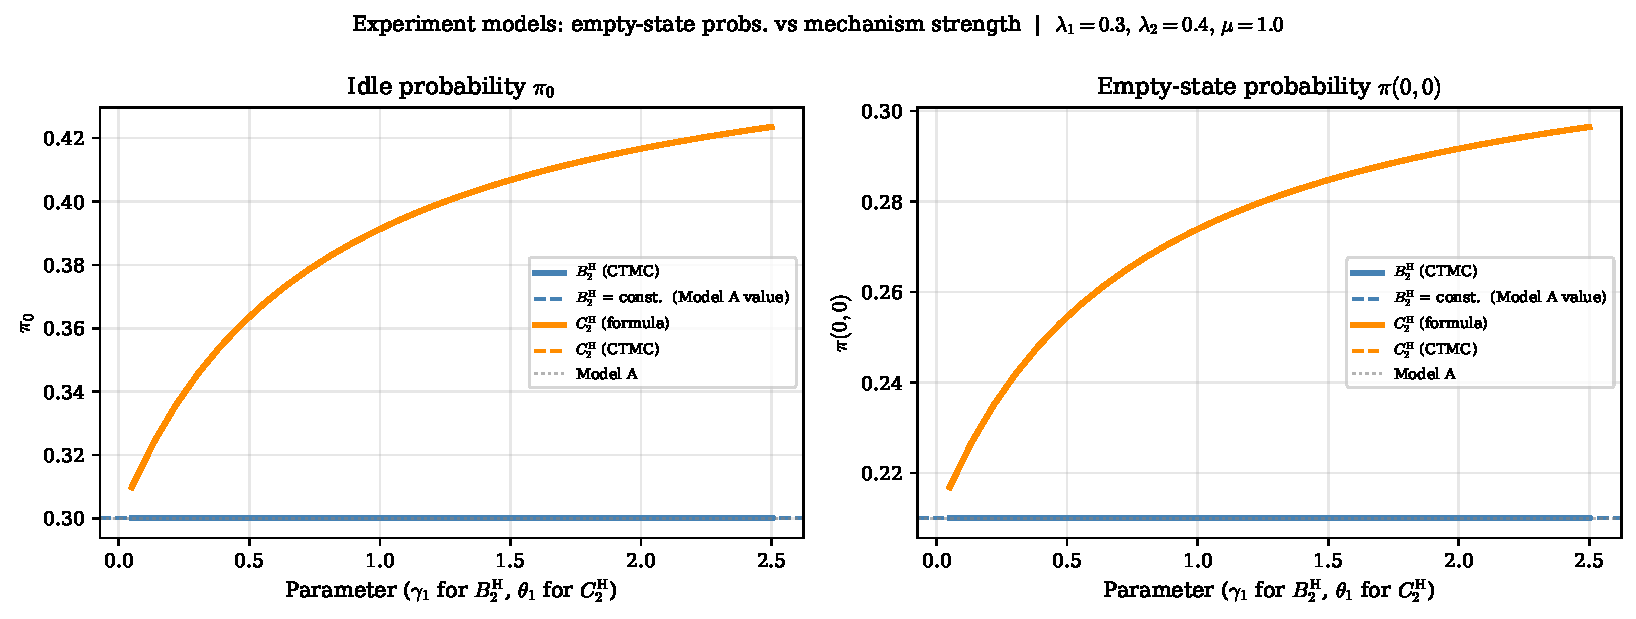
\includegraphics[width=0.85\textwidth]{figures/validation/val_experiment_pi.pdf}
    \caption{Empty-state probabilities $\pi_0$ and $\pi(0,0)$ as the mechanism
    parameter increases from $0$ to $2.5$.
    \textit{Left}: $\BH$ (blue) maintains $\pi_0=1-\rho$ exactly for all
    $\gamma_1$ — jockeying conserves total customers.
    $\CH$ (orange) shows $\pi_0$ increasing with $\theta_1$: abandonment
    clears the priority queue faster, raising the server's idle fraction.
    \textit{Right}: same story for $\pi(0,0)$.
    Solid orange = closed-form formula~\eqref{eq:C21:pi0_pi00}; dashed orange
    = CTMC.  The two are indistinguishable (max error $<10^{-4}$).
    The flat $\BH$ line is a structural result, not merely a numerical
    observation: $\pi_0=1-\rho$ holds identically for every $\gamma_1$ by the
    conservation corollary.}
    \label{fig:val_experiment_pi}
\end{figure}

\subsubsection{Cross-verification: simulation versus the CTMC}
\label{subsec:results:crossval}

The CTMC solver is the analytical ground truth used throughout this work, but it is
itself a numerical object: it solves $\pi Q=0$ on a finite truncation of the state space.
As an independent check, the stationary distribution is also estimated by a discrete-event
simulation of the master Markov chain, driven by the same rate structure but making no
truncation and no linear-algebra assumption. Figure~\ref{fig:results:crossval} plots, for
each canonical model, the CTMC value $\pi(n_1,n_2)$ against the simulated frequency for
every state with $\pi(n_1,n_2)>10^{-4}$.

%% BEGIN SIMULATION RESULTS — fig_sim_vs_ctmc %%
\begin{figure}[H]
  \centering
  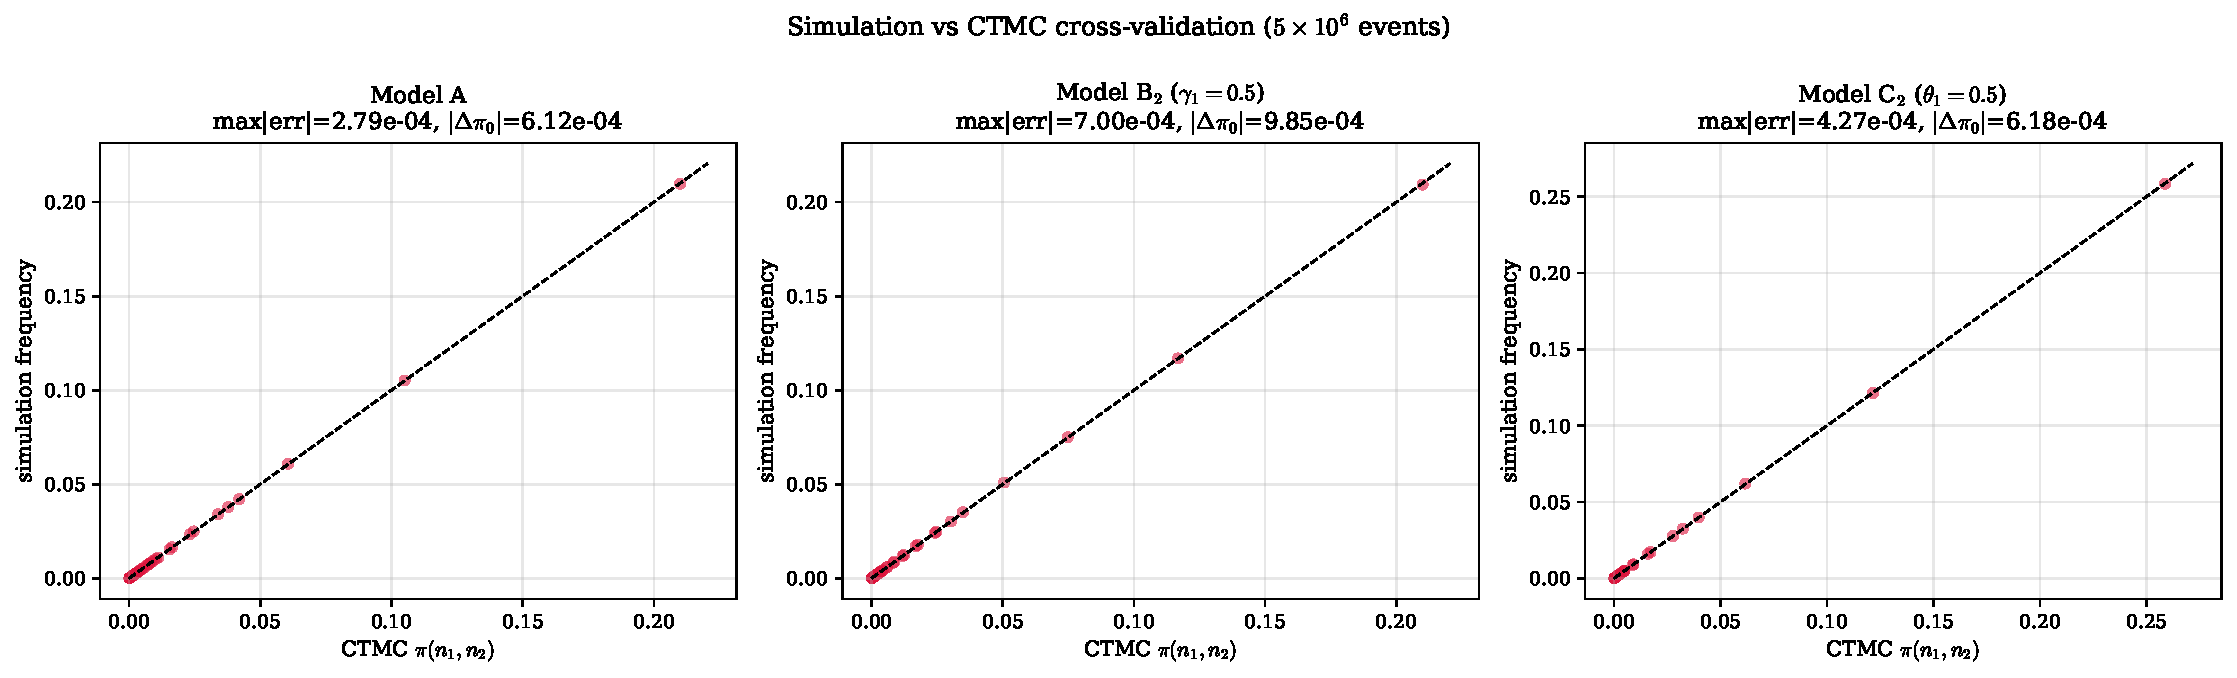
\includegraphics[width=0.98\textwidth]{figures/results/fig_sim_vs_ctmc.pdf}
  \caption{Simulation versus exact CTMC for Models $A$, $B_2$ ($\gamma_1=0.5$) and $C_2$
  ($\theta_1=0.5$) at $\lambda_1=0.3$, $\lambda_2=0.4$, $\mu=1$. Each point is one state
  $(n_1,n_2)$; the dashed line is $y=x$. The simulation uses $5\times10^6$ events (lower
  precision than the CTMC), yet every point lies on the diagonal, with maximum absolute
  discrepancy below $10^{-2}$ for all three models.}
  \label{fig:results:crossval}
\end{figure}
%% END SIMULATION RESULTS — fig_sim_vs_ctmc %%

The points cluster tightly on the $y=x$ line in all three panels, and the maximum absolute
deviation between the two independent computations is below $10^{-2}$ throughout --- the
residual being entirely consistent with the $O(1/\sqrt{n})$ sampling error of a
$5\times10^6$-event run. The two methods agree on $\pi_0$ to the same order. This closes the
verification loop: the closed-form expressions match the CTMC (\S\ref{subsec:validation} and
Table~\ref{tab:validation_summary}), and the CTMC matches an assumption-free simulation,
so the analytical formulas are verified against a fully independent estimator.

The same cross-check is run for the two head-of-line experiment models, whose CTMC carries a
\emph{constant} class-1 mechanism rate $\gamma_1\mathbf{1}_{\{n_1\ge1\}}$ or
$\theta_1\mathbf{1}_{\{n_1\ge1\}}$ rather than the length-proportional $\gamma_1 n_1$ or
$\theta_1 n_1$ of $B_2$, $C_2$. Both the event-driven simulator and the truncated solver
honour this head-of-line rate, so Figure~\ref{fig:results:crossval_exp} is an independent
test of the new transition structure underlying Models~$\BH$ and~$\CH$.

%% BEGIN SIMULATION RESULTS — fig_sim_vs_ctmc_experiment %%
\begin{figure}[H]
  \centering
  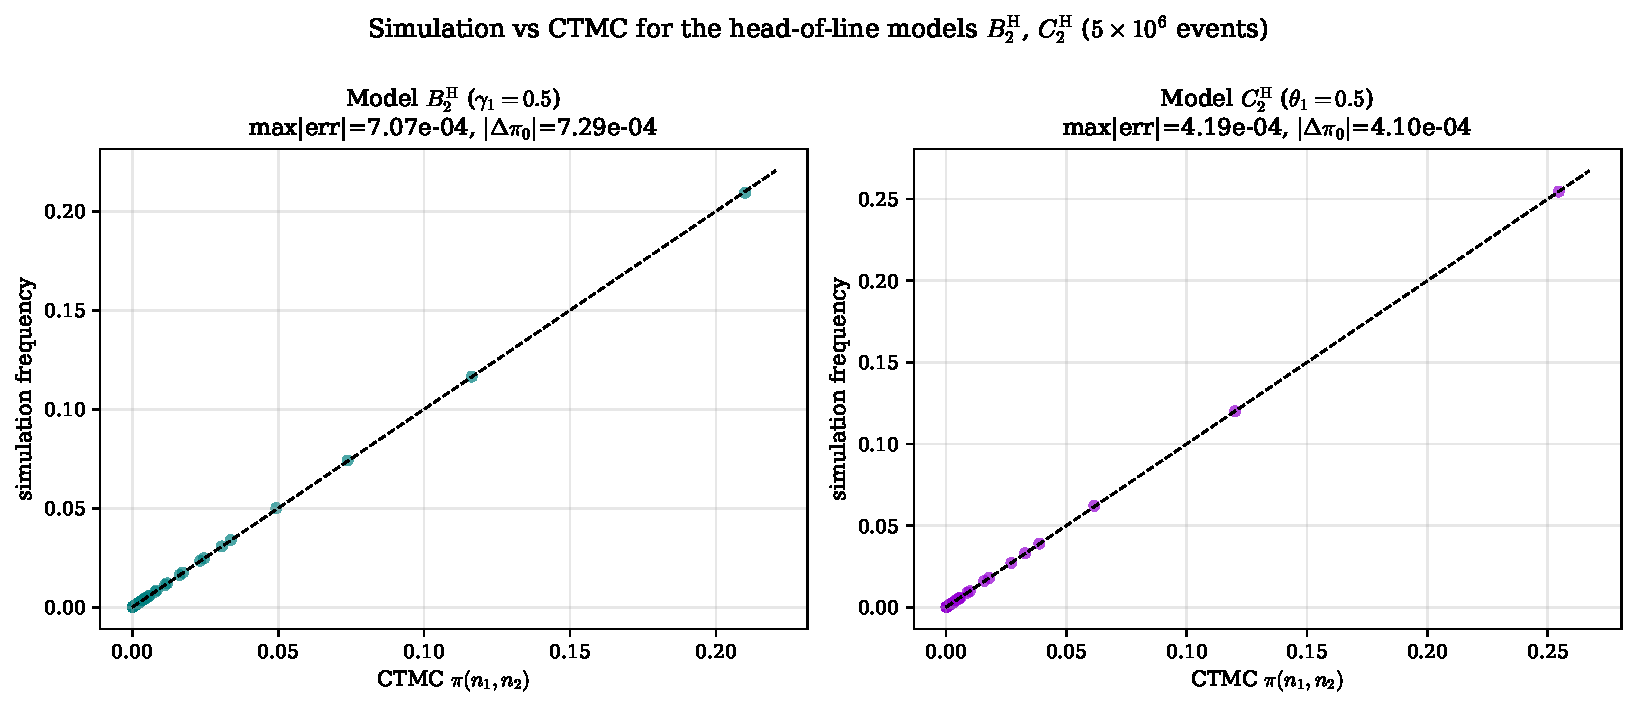
\includegraphics[width=0.82\textwidth]{figures/results/fig_sim_vs_ctmc_experiment.pdf}
  \caption{Simulation versus exact CTMC for the head-of-line models $\BH$
  ($\gamma_1=0.5$) and $\CH$ ($\theta_1=0.5$) at $\lambda_1=0.3$, $\lambda_2=0.4$,
  $\mu=1$. Each point is one state $(n_1,n_2)$; the dashed line is $y=x$. As for the
  full-rate models, every point lies on the diagonal, with maximum absolute discrepancy
  below $10^{-2}$, confirming that the constant-rate $\mathbf{1}_{\{n_1\ge1\}}$ transition is
  implemented consistently in both the simulator and the solver.}
  \label{fig:results:crossval_exp}
\end{figure}
%% END SIMULATION RESULTS — fig_sim_vs_ctmc_experiment %%

% =====================================================================
\subsection{Extended traffic-intensity and mechanism sweeps}\label{app:numerics:sweep}

This subsection expands the quantitative comparison of \S\ref{subsec:comp:sweep}: the
$\pi(0,0)$ sweep, the companion loss-accounting and queue-length tables, the isolated
jockeying and abandonment sweeps, the class-asymmetry study, the priority-benefit contrast,
and the head-of-line versus full-rate comparison.

\subsubsection{The busy-but-empty probability \texorpdfstring{$\pi(0,0)$}{pi(0,0)}}

%% BEGIN SIMULATION RESULTS — fig_sweep_pi00_vs_rho %%
\begin{figure}[H]
  \centering
  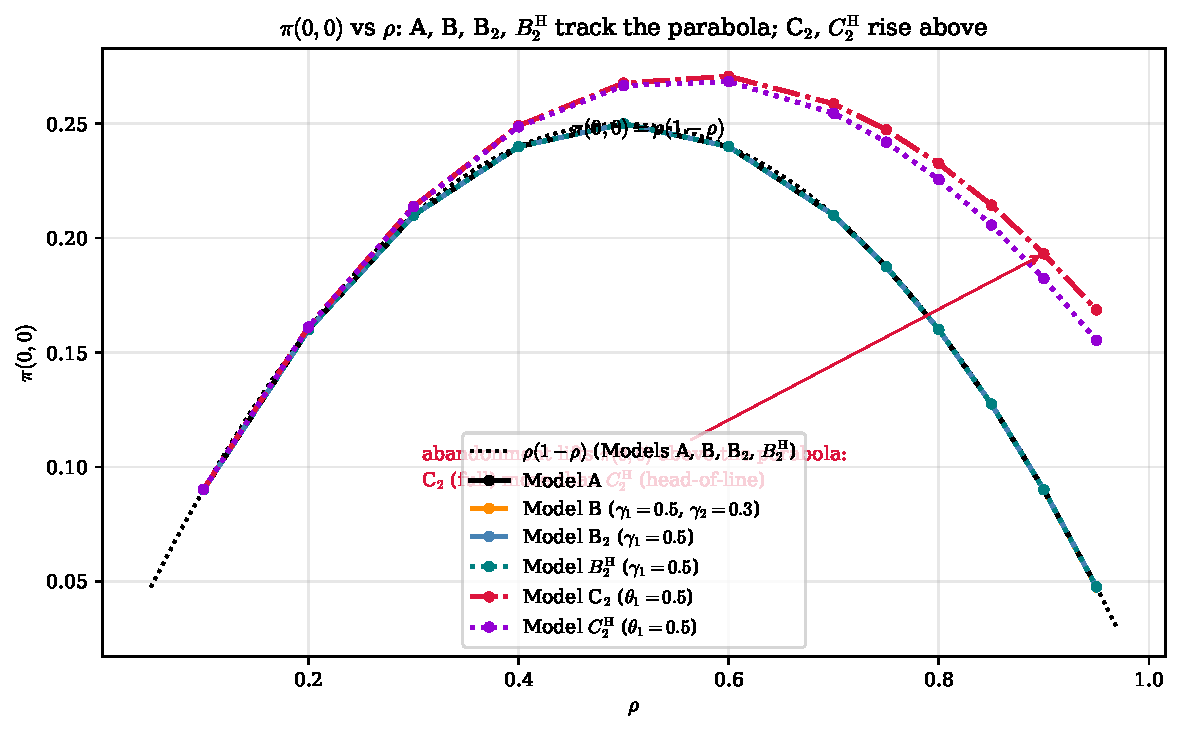
\includegraphics[width=0.78\textwidth]{figures/results/fig_sweep_pi00_vs_rho.pdf}
  \caption{$\pi(0,0)$ versus $\rho$. The three customer-conserving models $A$, $B_2$ and
  $\BH$ lie exactly on the parabola $\rho(1-\rho)$ (Corollaries~\ref{cor:A:pi0},
  \ref{cor:B2:pi00}, \ref{cor:B21:pi0}: jockeying preserves $N$, hence the busy-but-empty
  probability), whereas the abandonment models $C_2$ and $\CH$ rise strictly above it ---
  abandonment inflates $\pi(0,0)$ through the enlarged idle probability $\pi(0,0)=\rho\,\pi_0$
  (Corollaries~\ref{cor:C2:pi00}, \ref{cor:C21:pi0}), the full rate ($C_2$) lifting it more
  than the head-of-line rate ($\CH$).}
  \label{fig:comp:pi00}
\end{figure}
%% END SIMULATION RESULTS — fig_sweep_pi00_vs_rho %%

The invariance of $\pi(0,0)=\rho(1-\rho)$ along the $A$ and $B_2$ curves of
Figure~\ref{fig:comp:pi00} is not a numerical coincidence but a direct reading of
Corollary~\ref{cor:B2:pi00}: the event ``server busy, both queues empty'' depends only on
the total occupancy $N$, and jockeying leaves the law of $N$ unchanged. For $C_2$ the
identity $\pi(0,0)=\rho\,\pi_0$ still holds, but $\pi_0>1-\rho$, so the curve is lifted ---
at $\rho=0.70$, $\pi(0,0)=\piZZCtwoSeventy$ against the baseline $\piZZASeventy$
(Table~\ref{tab:comp:main}). The lift is also asymmetric: whereas the conserving parabola
$\rho(1-\rho)$ is symmetric about $\rho=\tfrac12$, the $C_2$ curve in
Figure~\ref{fig:comp:pi00} attains its maximum to the \emph{right} of that point, the
signature of abandonment renormalising the effective load --- the busy-but-empty probability
keeps climbing past the symmetric-load peak because the self-regulating valve blunts
congestion fastest exactly where the baseline is heaviest, before the shrinking busy fraction
finally pulls it down.

\subsubsection{Companion loss-accounting and queue-length tables}

The class-1 loss accounting that accompanies Table~\ref{tab:comp:main} is collected in
Table~\ref{tab:comp:loss_acct}: in every row the carried throughput and the abandonment
rate sum to the offered load $\rho$, and only the abandonment models $C_2$ and $\CH$ carry a
positive loss fraction $L_1$.

% Companion loss-accounting table. Hand-authored but every number is sourced from
% results/derived_metrics.tex (D1 pipeline); re-run Code/compute_derived_metrics.py to
% regenerate the macros. Kept separate from Table~\ref{tab:comp:main} to stay within margins.
\begin{table}[H]\centering
\caption{Class-1 loss accounting accompanying Table~\ref{tab:comp:main}, at the same three
loads and parameters ($\lambda_1{:}\lambda_2=3{:}4$, $\mu=1$; mechanism parameter $0.5$).
\emph{Throughput} is the carried rate $\mu(1-\pi_0)$; \emph{abandonment rate} is the class-1
loss flow ($\theta_1\mathbb{E}[N_1]$ for the full rate, $\theta_1\mathbb{P}(N_1\ge1)$ for
head-of-line); and $L_1=\theta_1\mathbb{E}[N_1]/\lambda_1$ is the fraction
of class-1 arrivals shed before service (eq.~\eqref{eq:comp:lossfrac}). The conserving models
$A$, $B_2$, $\BH$ lose nothing; only $C_2$ and $\CH$ have $L_1>0$, and at
every row throughput${}+{}$abandonment rate${}={}$offered load $\rho$.}
\label{tab:comp:loss_acct}
\begin{tabular}{llrrr}
\toprule
$\rho$ & Model & Throughput & Aband.\ rate & $L_1$ \\
\midrule
\multirow{5}{*}{0.50} & A & \throughputAFifty & $0$ & $0$ \\
 & B$_2$ & \throughputBtwoFifty & $0$ & $0$ \\
 & $\BH$ & \throughputBHFifty & $0$ & $0$ \\
 & C$_2$ & \throughputCtwoFifty & \lostflowCtwoFifty & \lossCtwoFifty \\
 & $\CH$ & \throughputCHFifty & \lostflowCHFifty & \lossCHFifty \\
\midrule
\multirow{5}{*}{0.70} & A & \throughputASeventy & $0$ & $0$ \\
 & B$_2$ & \throughputBtwoSeventy & $0$ & $0$ \\
 & $\BH$ & \throughputBHSeventy & $0$ & $0$ \\
 & C$_2$ & \throughputCtwoSeventy & \lostflowCtwoSeventy & \lossCtwoSeventy \\
 & $\CH$ & \throughputCHSeventy & \lostflowCHSeventy & \lossCHSeventy \\
\midrule
\multirow{5}{*}{0.90} & A & \throughputANinety & $0$ & $0$ \\
 & B$_2$ & \throughputBtwoNinety & $0$ & $0$ \\
 & $\BH$ & \throughputBHNinety & $0$ & $0$ \\
 & C$_2$ & \throughputCtwoNinety & \lostflowCtwoNinety & \lossCtwoNinety \\
 & $\CH$ & \throughputCHNinety & \lostflowCHNinety & \lossCHNinety \\
\bottomrule
\end{tabular}
\end{table}

%% BEGIN SIMULATION RESULTS — tab_EN_sweep %%
\begin{table}[t]\centering
\caption{Class-1 mean queue length $E[N_1]$ and waiting time $E[W_1]$ under Models A, B$_2$ ($\gamma_1=0.5$) and C$_2$ ($\theta_1=0.5$), with $\mu=1$ and $\lambda_1{:}\lambda_2=3{:}4$.}
\label{tab:comp:EN_sweep}
\begin{tabular}{lrrrrrr}
\toprule
 & \multicolumn{3}{c}{$E[N_1]$} & \multicolumn{3}{c}{$E[W_1]$} \\
\cmidrule(lr){2-4}\cmidrule(lr){5-7}
$\rho$ & A & B$_2$ & C$_2$ & A & B$_2$ & C$_2$ \\
\midrule
0.50 & 0.1364 & 0.0767 & 0.0712 & 0.6364 & 0.3578 & 0.3323 \\
0.70 & 0.3000 & 0.1545 & 0.1392 & 1.0000 & 0.5151 & 0.4639 \\
0.90 & 0.5651 & 0.2626 & 0.2292 & 1.4651 & 0.6808 & 0.5941 \\
\bottomrule
\end{tabular}
\end{table}

%% END SIMULATION RESULTS — tab_EN_sweep %%

Table~\ref{tab:comp:EN_sweep} reads off the per-class queue lengths and waiting times across
the sweep. The priority waiting time $\mathbb{E}[W_1]$ is smallest for $C_2$ at every load
($\EWoneCtwoNinety$ at $\rho=0.90$ against $\EWoneBtwoNinety$ for $B_2$ and $\EWoneANinety$ for $A$), but
$\mathbb{E}[W_i]=\mathbb{E}[N_i]/\lambda_i$ is the mean time a customer is \emph{counted in
queue~$i$}, and that residence is shortened by every departure mode --- service,
\emph{and} attrition. In $C_2$ a class-1 customer leaves the count by being served
\emph{or} by abandoning; in $B_2$ by being served \emph{or} by jockeying into class~2.
A smaller $\mathbb{E}[W_1]$ therefore does not by itself certify faster service, and
cross-model $\mathbb{E}[W_1]$ comparisons conflate latency reduction with customer loss; the
loss fraction $L_1$ of \S\ref{subsec:comp:abandonment} measures exactly the size of that
confound.

\subsubsection{The jockeying mechanism (Model \texorpdfstring{$B_2$}{B2})}
\label{subsec:comp:jockeying}

Figure~\ref{fig:b2:jockeying} isolates the action of $\gamma_1$ at fixed load $\rho=0.70$,
sweeping $\gamma_1\in[10^{-3},50]$.

%% BEGIN SIMULATION RESULTS — fig_B2_jockeying_EN_vs_gamma1 %%
\begin{figure}[H]
  \centering
  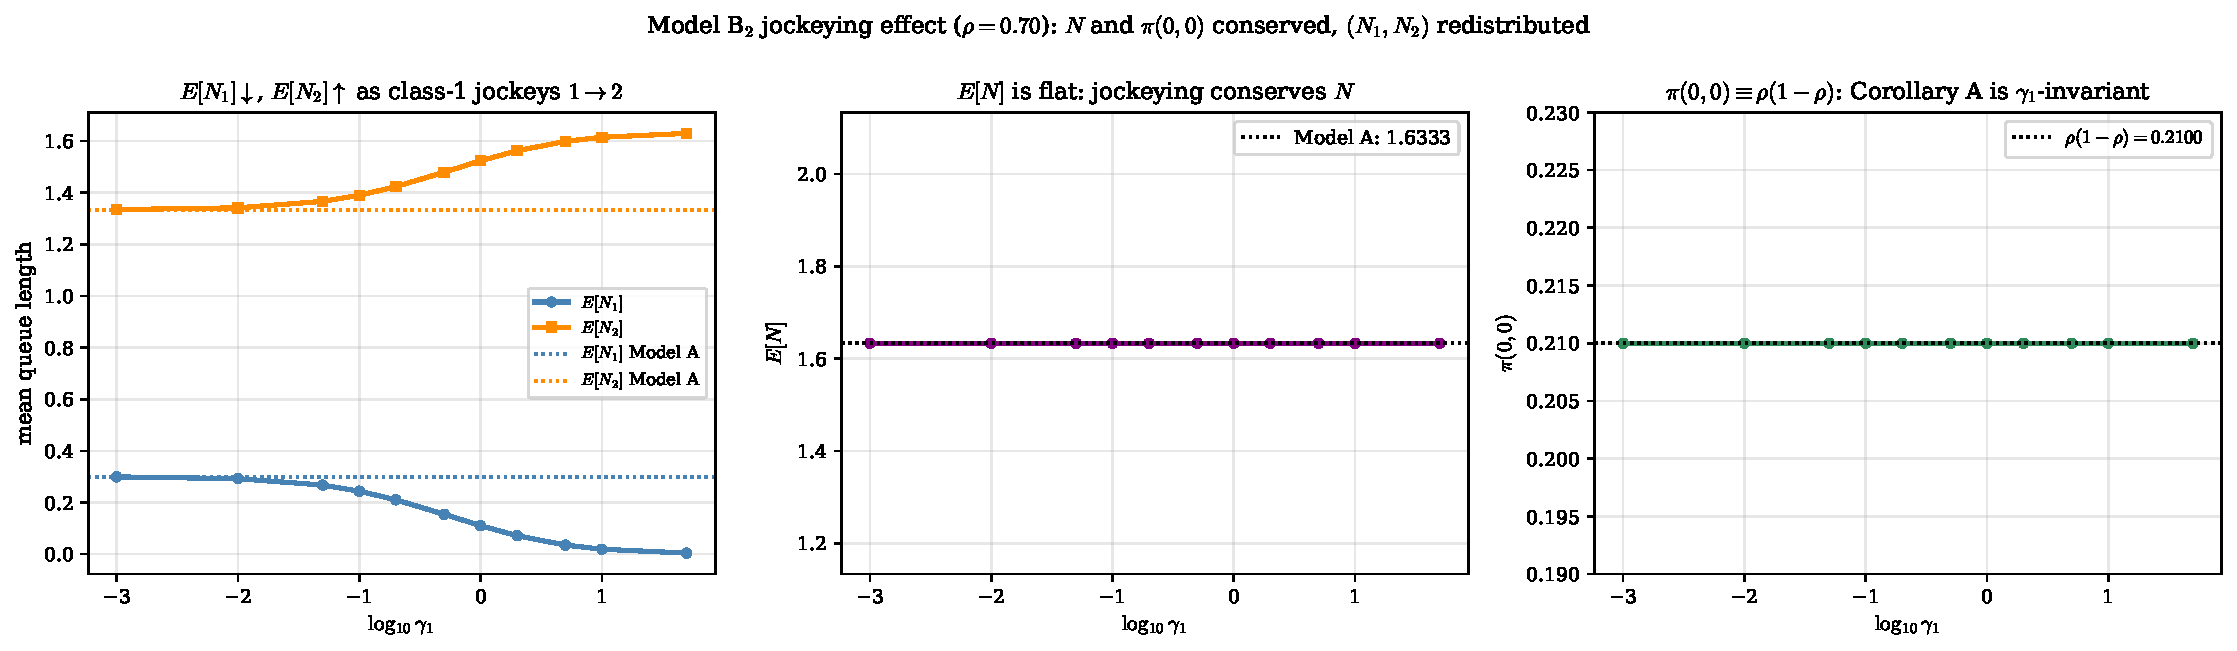
\includegraphics[width=0.98\textwidth]{figures/results/fig_B2_jockeying_EN_vs_gamma1.pdf}
  \caption{Model-$B_2$ at $\rho=0.70$ ($\lambda_1=0.3$, $\lambda_2=0.4$, $\mu=1$).
  \emph{Left:} $\mathbb{E}[N_1]$ decreases and $\mathbb{E}[N_2]$ increases monotonically in
  $\gamma_1$ (Model-$A$ values dotted). \emph{Centre:} $\mathbb{E}[N]$ is flat ---
  jockeying conserves the total count. \emph{Right:} $\pi(0,0)\equiv\rho(1-\rho)=0.21$ for
  all $\gamma_1$, the numerical signature of Corollary~\ref{cor:B2:pi00}.}
  \label{fig:b2:jockeying}
\end{figure}
%% END SIMULATION RESULTS — fig_B2_jockeying_EN_vs_gamma1 %%

The monotone decrease of $\mathbb{E}[N_1]$ in $\gamma_1$ follows directly from the rate
structure: each waiting class-1 customer generates a jockeying event at rate $\gamma_1$, so
the expected outflow from the class-1 queue is $\gamma_1\mathbb{E}[N_1]$, an additional
drain that acts independently of the service process and grows with $\gamma_1$. At
$\gamma_1=0.5$ this halves the priority queue, from $\mathbb{E}[N_1]=\ENoneASeventy$ to $\ENoneBtwoSeventy$
($-\ENoneBtwoReductionSeventy\%$, Table~\ref{tab:comp:main}). The mass is not destroyed but transferred:
$\mathbb{E}[N_2]$ rises correspondingly from $\ENtwoASeventy$ to $\ENtwoBtwoSeventy$, and the centre panel
confirms $\mathbb{E}[N]=\ENASeventy$ is held constant to plotting precision. The right panel is
the cleanest empirical check of Corollary~\ref{cor:B2:pi00}: because every jockeying
transition preserves $N$, the load on the server --- and therefore $\pi_0=1-\rho$ and
$\pi(0,0)=\rho(1-\rho)=0.21$ --- is exactly $\gamma_1$-invariant.

%% BEGIN SIMULATION RESULTS — fig_B2_priority_ratio_vs_gamma1 %%
\begin{figure}[H]
  \centering
  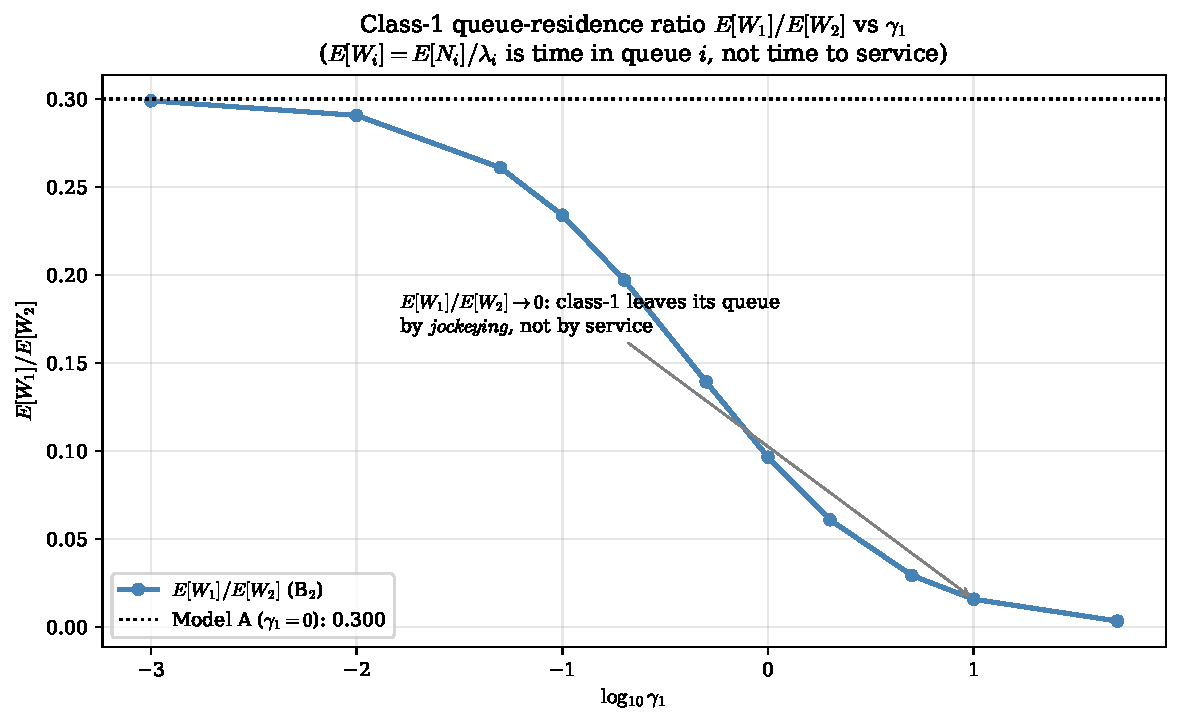
\includegraphics[width=0.80\textwidth]{figures/results/fig_B2_priority_ratio_vs_gamma1.pdf}
  \caption{Class-1 queue-residence ratio $\mathbb{E}[W_1]/\mathbb{E}[W_2]$ versus
  $\gamma_1$ at $\rho=0.70$, with the Model-$A$ value dotted. The ratio decreases toward
  zero because $\mathbb{E}[W_1]=\mathbb{E}[N_1]/\lambda_1$ measures time spent in the
  class-1 queue, which the jockeying drain $\gamma_1\mathbb{E}[N_1]$ collapses; it does not
  measure time to service.}
  \label{fig:b2:priority}
\end{figure}
%% END SIMULATION RESULTS — fig_B2_priority_ratio_vs_gamma1 %%

Figure~\ref{fig:b2:priority} must be read with the residence-time caveat of
\S\ref{subsec:comp:sweep} firmly in mind. As $\gamma_1$ grows the ratio
$\mathbb{E}[W_1]/\mathbb{E}[W_2]$ falls monotonically from the Model-$A$ value of $0.300$
toward zero, which would naively suggest an ever-improving class-1 service. The mechanism
is the opposite: a large $\gamma_1$ ejects class-1 customers from their own queue almost
immediately, so the \emph{count} $\mathbb{E}[N_1]$ and hence $\mathbb{E}[W_1]$ vanish, but
the ejected customers simply wait out their delay at the back of the class-2 queue. The
falling ratio records the dissolution of the class-1 queue, not an acceleration of class-1
service. This is the precise sense in which strong one-way jockeying \emph{erodes the
priority structure}: in the limit there is effectively a single class.

\subsubsection{Class asymmetry}
\label{subsec:comp:asymmetry}

Fixing $\rho=0.70$ and varying the split $\alpha=\lambda_1/(\lambda_1+\lambda_2)$ exposes
how the mechanisms interact with the class mix. Figure~\ref{fig:comp:asymmetry} compares the
three models; Figure~\ref{fig:b2:asymmetry} resolves the jockeying case at three rates.

%% BEGIN SIMULATION RESULTS — fig_class_asymmetry %%
\begin{figure}[H]
  \centering
  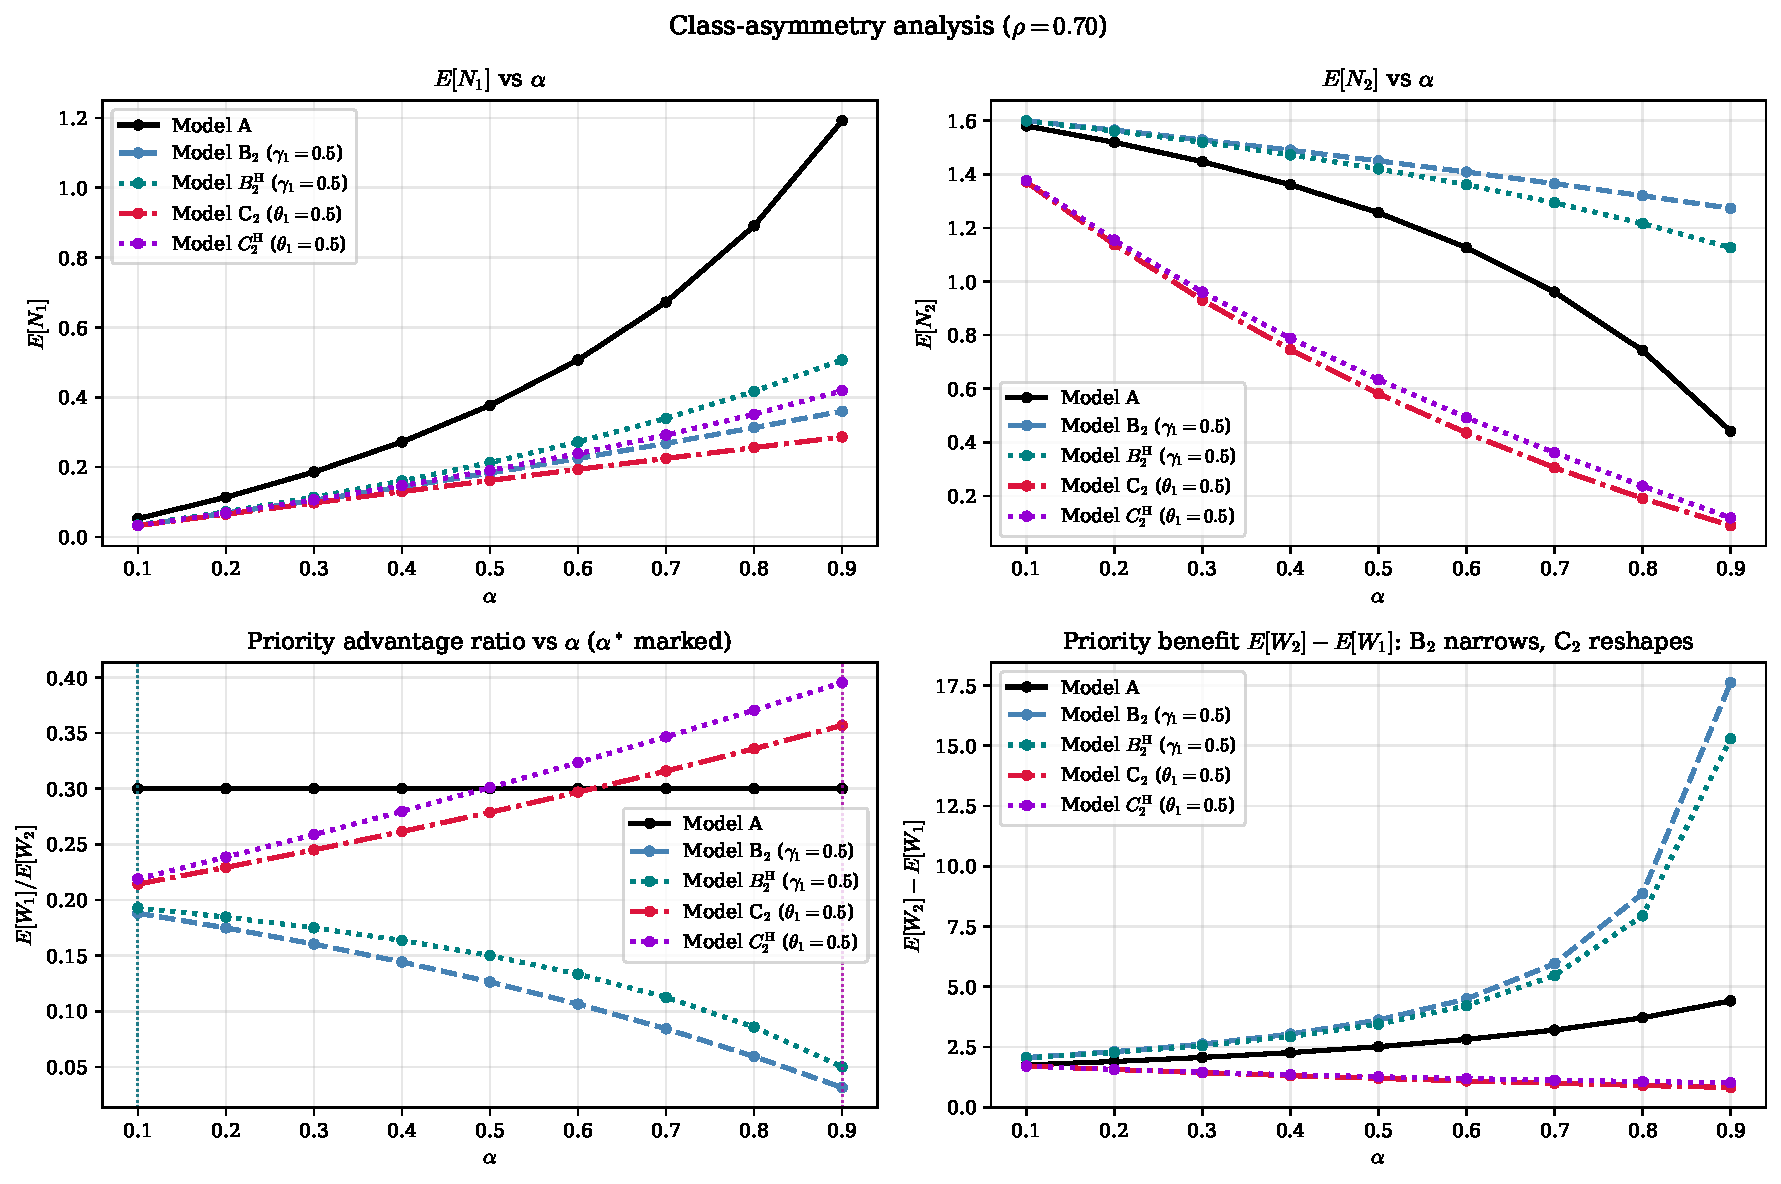
\includegraphics[width=0.98\textwidth]{figures/results/fig_class_asymmetry.pdf}
  \caption{Class-asymmetry sweep at $\rho=0.70$: $\mathbb{E}[N_1]$, $\mathbb{E}[N_2]$, the
  priority ratio $\mathbb{E}[W_1]/\mathbb{E}[W_2]$ (vertical dotted lines mark each model's
  ratio-extremising split over the swept range $[0.1,0.9]$), and the absolute priority
  benefit $\mathbb{E}[W_2]-\mathbb{E}[W_1]$, for Models $A$, $B_2$ and $\BH$
  ($\gamma_1=0.5$), and $C_2$ and $\CH$ ($\theta_1=0.5$).}
  \label{fig:comp:asymmetry}
\end{figure}
%% END SIMULATION RESULTS — fig_class_asymmetry %%

As $\alpha\to0$ the priority class is vanishingly rare and its mechanism barely engages:
all models converge in $\mathbb{E}[N_1]$. As $\alpha\to1$ the priority class
dominates the offered load and the non-preemptive discipline gives it near-exclusive access
to the server, driving $\mathbb{E}[N_1]\to0$ in every model. The interesting behaviour is
interior. The absolute priority benefit $\mathbb{E}[W_2]-\mathbb{E}[W_1]$ (bottom-right) is
largest where class~2 bears the most displaced load; jockeying narrows this gap relative to
$A$ by exporting class-1 delay into the class-2 statistic, while abandonment reshapes it by
removing class-1 work outright.

The priority ratio $\mathbb{E}[W_1]/\mathbb{E}[W_2]$ (bottom-left) carries the sharpest
structural signal. For Model-$A$ it is \emph{exactly $\alpha$-invariant}: writing the ratio
as $\mathbb{E}[W_1]/\mathbb{E}[W_2]=(\mathbb{E}[N_1]\,\lambda_2)/(\mathbb{E}[N_2]\,\lambda_1)$
and substituting the closed forms $\mathbb{E}[N_1]=\rho\rho_1/(1-\rho_1)$ and
$\mathbb{E}[N]=\rho^2/(1-\rho)$ collapses the split dependence entirely,
\begin{equation*}
  \left.\frac{\mathbb{E}[W_1]}{\mathbb{E}[W_2]}\right|_{A}=1-\rho
  \qquad\text{for every }\alpha\in(0,1),
\end{equation*}
the flat line at $\ratioPeakA=1-\rho$ in the panel. The two mechanisms break this invariance
in \emph{opposite, monotone} directions. Jockeying makes the ratio strictly \emph{decreasing}
in $\alpha$, so it peaks at $\ratioPeakBtwo$ at the left endpoint $\alpha^\ast=\alphaStarBtwo$
(a larger priority share feeds the $1\!\to\!2$ drain harder); abandonment makes it strictly
\emph{increasing}, peaking at $\ratioPeakCtwo$ at the right endpoint
$\alpha^\ast=\alphaStarCtwo$ (a larger priority share is exactly where the abandonment valve
sheds the most class-1 work). The head-of-line variants track their parents --- $\BH$ peaks at
$\ratioPeakBH$ ($\alpha^\ast=\alphaStarBH$) and $\CH$ at $\ratioPeakCH$
($\alpha^\ast=\alphaStarCH$) --- and are likewise monotone. No curve turns over: across all
five models the maximiser $\alpha^\ast$ sits at a \emph{boundary} of the swept range
$[0.1,0.9]$, never at an interior point. An interior $\alpha^\ast$ would require mechanism
engagement (which strengthens as the priority class grows) to balance class dominance at some
intermediate split; here the two effects pull the ratio the same way throughout, so the
extremum is always pushed to an endpoint.

%% BEGIN SIMULATION RESULTS — fig_B2_class_asymmetry_gamma1 %%
\begin{figure}[H]
  \centering
  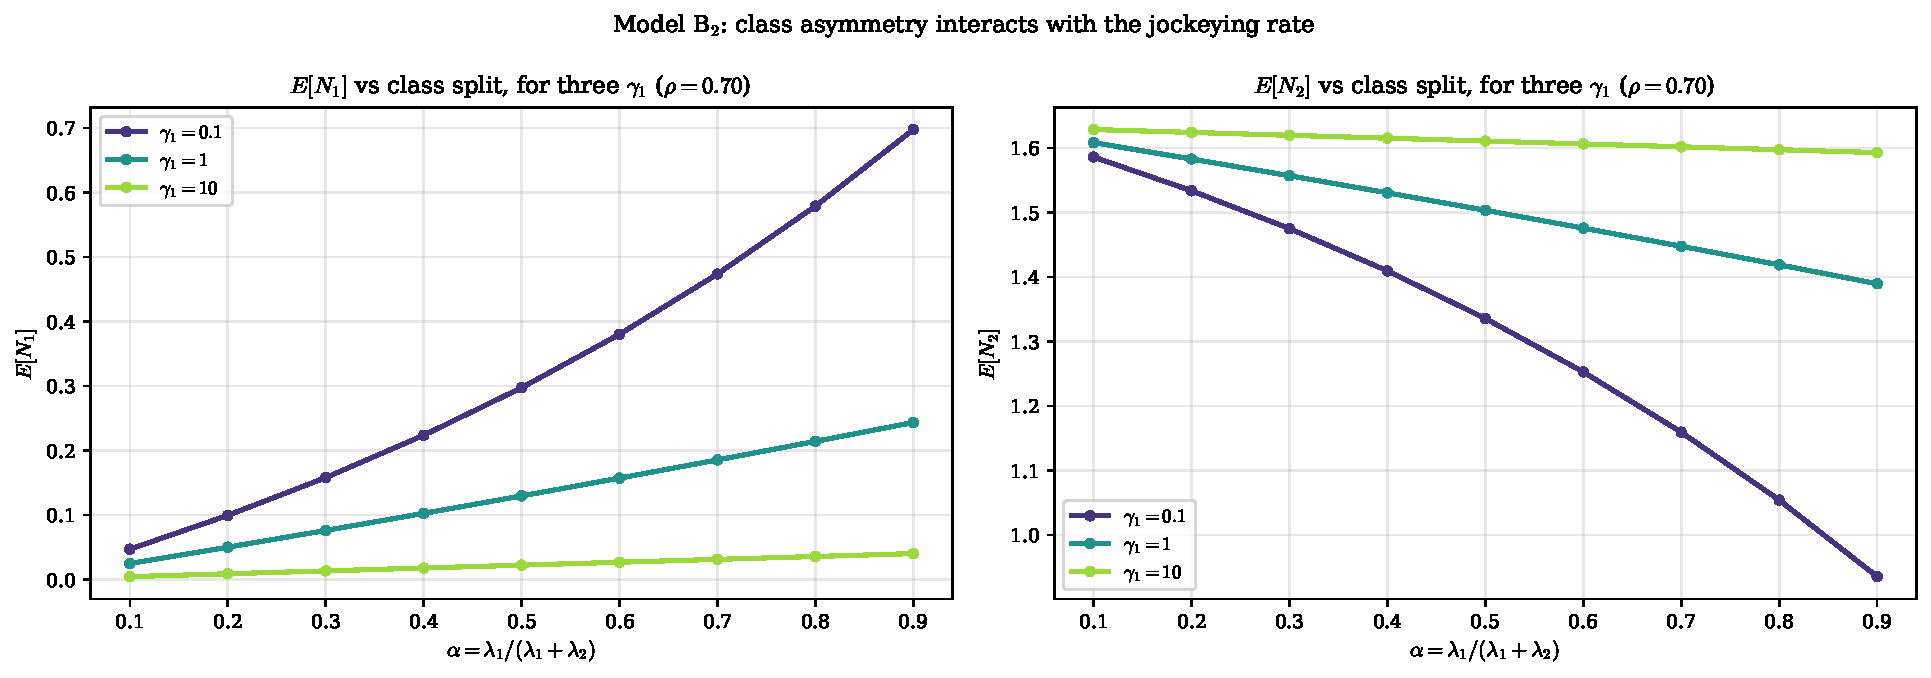
\includegraphics[width=0.98\textwidth]{figures/results/fig_B2_class_asymmetry_gamma1.pdf}
  \caption{Model-$B_2$: $\mathbb{E}[N_1]$ and $\mathbb{E}[N_2]$ versus the split $\alpha$
  for three jockeying rates $\gamma_1\in\{0.1,1.0,10.0\}$ at $\rho=0.70$. Stronger
  jockeying flattens $\mathbb{E}[N_1]$ toward zero across the whole range of $\alpha$ and
  loads the difference onto $\mathbb{E}[N_2]$.}
  \label{fig:b2:asymmetry}
\end{figure}
%% END SIMULATION RESULTS — fig_B2_class_asymmetry_gamma1 %%

The family in Figure~\ref{fig:b2:asymmetry} shows that the jockeying drain dominates the
class mix: at $\gamma_1=10$ the priority queue is essentially empty for every $\alpha$,
because the per-customer ejection rate $\gamma_1$ overwhelms the arrival rate $\lambda_1$
regardless of the split. At $\gamma_1=0.1$ the curves still track the Model-$A$ shape, the
drain being a small perturbation. The crossover between these regimes occurs where
$\gamma_1$ is comparable to the effective class-1 service rate, consistent with the
singular role of $\gamma_1$ in the $B_2$ ODE.

\subsubsection{The abandonment mechanism (Model \texorpdfstring{$C_2$}{C2})}

Figure~\ref{fig:c2:abandonment} sweeps $\theta_1\in[10^{-3},50]$ at $\rho=0.70$.

%% BEGIN SIMULATION RESULTS — fig_C2_abandonment_EN_vs_theta1 %%
\begin{figure}[H]
  \centering
  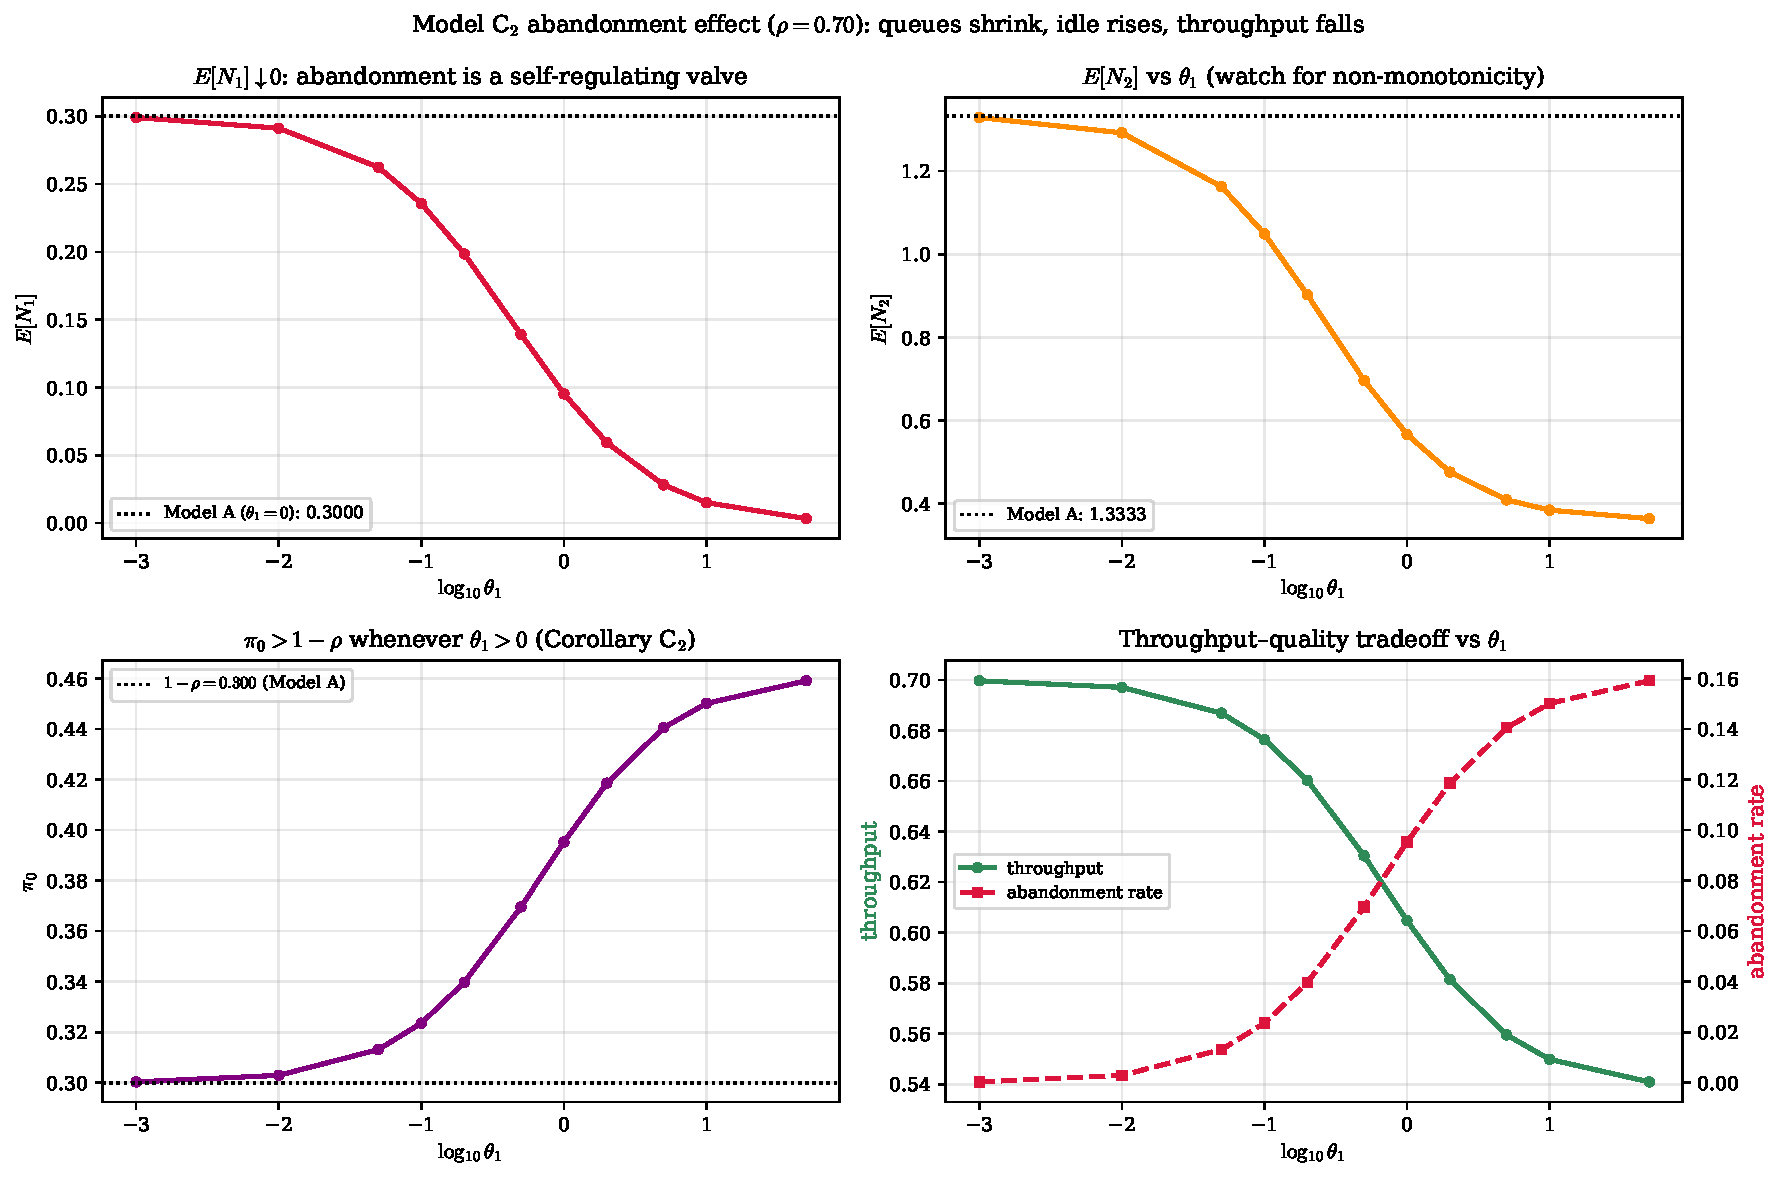
\includegraphics[width=0.98\textwidth]{figures/results/fig_C2_abandonment_EN_vs_theta1.pdf}
  \caption{Model-$C_2$ at $\rho=0.70$. \emph{Top-left:} $\mathbb{E}[N_1]\to0$ as the
  abandonment valve $\theta_1 n_1$ strengthens. \emph{Top-right:} $\mathbb{E}[N_2]$
  \emph{decreases monotonically} (no rebound at these parameters). \emph{Bottom-left:}
  $\pi_0>1-\rho$ for all $\theta_1>0$ (Corollary~\ref{cor:C2:pi00}). \emph{Bottom-right:}
  the throughput--quality tradeoff --- throughput falls and the abandonment rate rises with
  $\theta_1$.}
  \label{fig:c2:abandonment}
\end{figure}
%% END SIMULATION RESULTS — fig_C2_abandonment_EN_vs_theta1 %%

The priority queue $\mathbb{E}[N_1]$ collapses toward zero as $\theta_1$ grows: the
abandonment outflow $\theta_1\mathbb{E}[N_1]$ is a self-regulating valve that opens wider
the longer the queue, so no class-1 backlog can persist. The idle-probability panel is the
empirical face of Corollary~\ref{cor:C2:pi00}: every positive $\theta_1$ lifts $\pi_0$
strictly above the Model-$A$ value $1-\rho=0.30$, because customers who abandon never reach
the server and the busy fraction shrinks accordingly. This sweep also settles, as a
\emph{negative finding}, a question flagged in the simulation
brief. Two effects compete in $\mathbb{E}[N_2]$ as $\theta_1$ rises: abandonment is
class-1-specific, so clearing the priority backlog lets the server reach class~2 sooner --- an
effect that could in principle make $\mathbb{E}[N_2]$ rise transiently before falling --- set
against the plain reduction in the total work the class-2 queue inherits once class~1 is bled
off faster. At $\rho=0.70$ the second effect dominates throughout: $\mathbb{E}[N_2]$ is
\emph{monotonically decreasing} in $\theta_1$ with no initial hump, contradicting the
conjectured non-monotonicity. We observed no rebound at any load tested and conjecture that
$\mathbb{E}[N_2]$ is monotone decreasing in $\theta_1$ for every $\rho<1$; a proof, or a
counterexample at extreme class asymmetry, is left to future work (\S\ref{sec:future_work}).
The bottom-right panel quantifies the price and, in doing so, supplies an independent
numerical check. Throughput falls from the Model-$A$ value $\mu\rho=\offeredSeventy$ to
$\throughputCtwoSeventy$ at $\theta_1=0.5$, a deficit of $\lostflowCtwoSeventy$; computed
\emph{separately} as the abandonment flow $\theta_1\mathbb{E}[N_1]$, the lost rate reproduces
that same $\lostflowCtwoSeventy$, so carried plus lost returns the offered $\offeredSeventy$.
Because the throughput deficit $\mu\rho-\mu(1-\pi_0)$ and the abandonment integral
$\theta_1\mathbb{E}[N_1]$ are distinct functionals of the stationary law --- one read from the
idle probability of Corollary~\ref{cor:C2:pi00}, the other from the mean queue length --- their
agreement is not a restatement of flow balance but an independent verification of both.

%% BEGIN SIMULATION RESULTS — fig_C2_E_BC_vs_theta1 %%
\begin{figure}[H]
  \centering
  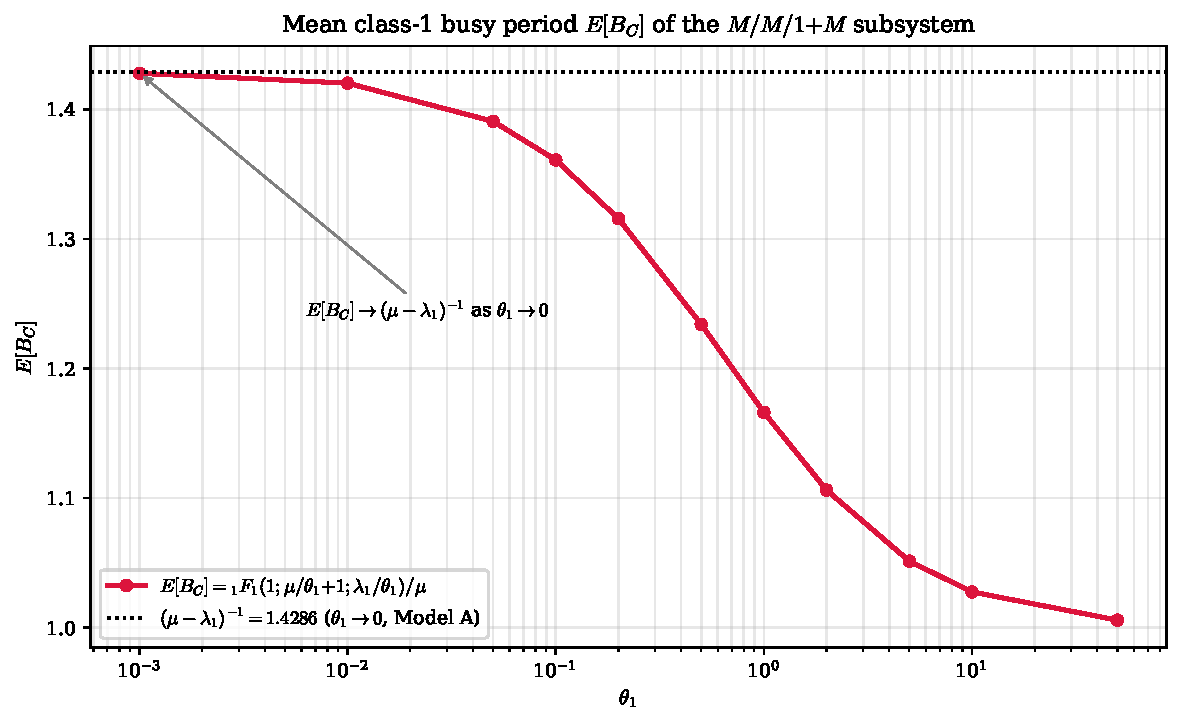
\includegraphics[width=0.78\textwidth]{figures/results/fig_C2_E_BC_vs_theta1.pdf}
  \caption{Mean class-1 busy period $\mathbb{E}[B_C]$ of the $M/M/1{+}M$ subsystem versus
  $\theta_1$, computed in closed form from
  $\mathbb{E}[B_C]={}_1F_1(1;\mu/\theta_1+1;\lambda_1/\theta_1)/\mu$
  (cf.\ \eqref{eq:comp:1F1}). The horizontal asymptote is the Model-$A$ busy period
  $(\mu-\lambda_1)^{-1}=1.4286$, attained as $\theta_1\to0^+$ (Corollary~\ref{cor:C2:pi00}
  limit).}
  \label{fig:c2:ebc}
\end{figure}
%% END SIMULATION RESULTS — fig_C2_E_BC_vs_theta1 %%

The busy-period curve in Figure~\ref{fig:c2:ebc} is the engine of the $C_2$ corollary: the
confluent hypergeometric ${}_1F_1(1;\mu/\theta_1+1;\lambda_1/\theta_1)$ of
\eqref{eq:comp:1F1} interpolates between the abandonment-free busy period and the
fast-clearance regime. As $\theta_1\to0^+$ the Kummer function tends to unity in the
relevant ratio and $\mathbb{E}[B_C]\to(\mu-\lambda_1)^{-1}=1.4286$, recovering the Model-$A$
class-1 busy period; as $\theta_1$ grows the busy period shortens because the server is
relieved by abandonment as well as by service.

\subsubsection{The priority benefit}

%% BEGIN SIMULATION RESULTS — tab_priority_benefit %%
\begin{table}[t]\centering
\caption{Class-1 mean waiting time $E[W_1]$ and priority ratio $E[W_2]/E[W_1]$ under each model ($\lambda_1{:}\lambda_2=3{:}4$, $\mu=1$, $\gamma_1=\theta_1=0.5$).}
\label{tab:prio:benefit}
\begin{tabular}{lrrrrrr}
\toprule
 & \multicolumn{2}{c}{Model A} & \multicolumn{2}{c}{Model B$_2$} & \multicolumn{2}{c}{Model C$_2$} \\
\cmidrule(lr){2-3}\cmidrule(lr){4-5}\cmidrule(lr){6-7}
$\rho$ & $E[W_1]$ & $E[W_2]/E[W_1]$ & $E[W_1]$ & $E[W_2]/E[W_1]$ & $E[W_1]$ & $E[W_2]/E[W_1]$ \\
\midrule
0.50 & 0.6364 & 2.0000 & 0.3578 & 4.1411 & 0.3323 & 2.6551 \\
0.70 & 1.0000 & 3.3333 & 0.5151 & 7.1774 & 0.4639 & 3.7545 \\
0.90 & 1.4651 & 9.9996 & 0.6808 & 22.3834 & 0.5941 & 6.2985 \\
\bottomrule
\end{tabular}
\end{table}

%% END SIMULATION RESULTS — tab_priority_benefit %%

Table~\ref{tab:prio:benefit} contrasts the priority structure directly. The ratio
$\mathbb{E}[W_2]/\mathbb{E}[W_1]$ measures how strongly the discipline favours class~1.
Jockeying inflates this ratio sharply --- to $\premiumBtwoSeventy$ at $\rho=0.70$ and
$\premiumBtwoNinety$ at $\rho=0.90$, against the baseline $\premiumASeventy$ and
$\premiumANinety$ --- but, as established in \S\ref{sec:comparison}, the inflation reflects the
collapse of the class-1 \emph{queue} (its residence time, not its service time) and a
simultaneous lengthening of class~2. Abandonment moves the ratio in the opposite direction at
high load ($\premiumCtwoNinety$ at $\rho=0.90$, below the baseline $\premiumANinety$), because
it compresses both waiting times by shedding load. The two mechanisms are thus not
substitutes: jockeying redistributes delay between classes at fixed total work, whereas
abandonment reduces total work at the cost of served throughput.

The $\rho=0.90$ row of Table~\ref{tab:prio:benefit} is the single sharpest statement of this
dichotomy. Under one and the same non-preemptive discipline the priority premium
$\mathbb{E}[W_2]/\mathbb{E}[W_1]$ moves to $\premiumBtwoNinety$ under jockeying and to
$\premiumCtwoNinety$ under abandonment, straddling the Model-$A$ baseline of $\premiumANinety$
in \emph{opposite} directions. Both models look ``better for class~1'' on the raw
$\mathbb{E}[W_1]$ column, yet for incompatible reasons --- jockeying widens the premium by
exporting class-1 delay onto class~2 at conserved total work, abandonment narrows it by
deleting class-1 work outright. Neither improvement is the naive one, faster service: reading
the premium without the loss fraction of \S\ref{subsec:comp:abandonment} would mistake
redistribution and attrition for speed.

\subsubsection{Head-of-line versus full-rate mechanisms (Models \texorpdfstring{$\BH$}{B2-H} and \texorpdfstring{$\CH$}{C2-H})}
\label{subsec:comp:hol}

The head-of-line models of \S\ref{sec:model_b21}--\ref{sec:model_c21} replace the
\emph{length-proportional} mechanism rate of $B_2$ and $C_2$ --- $\gamma_1 n_1$ or
$\theta_1 n_1$, in which every waiting class-1 customer participates --- by a
\emph{head-of-line} rate $\gamma_1\mathbf 1_{\{n_1\ge1\}}$ or $\theta_1\mathbf 1_{\{n_1\ge1\}}$,
in which only the customer at the head of Queue~1 may jockey or abandon. The aggregate
class-1 outflow is therefore capped at the single rate $\gamma_1$ (or $\theta_1$) instead of
growing with the queue, so each head-of-line mechanism is a strictly \emph{weaker} drain of
the priority queue than its full-rate counterpart. Figure~\ref{fig:comp:hol} quantifies the
gap at fixed load $\rho=0.70$.

%% BEGIN SIMULATION RESULTS — fig_hol_vs_full %%
\begin{figure}[H]
  \centering
  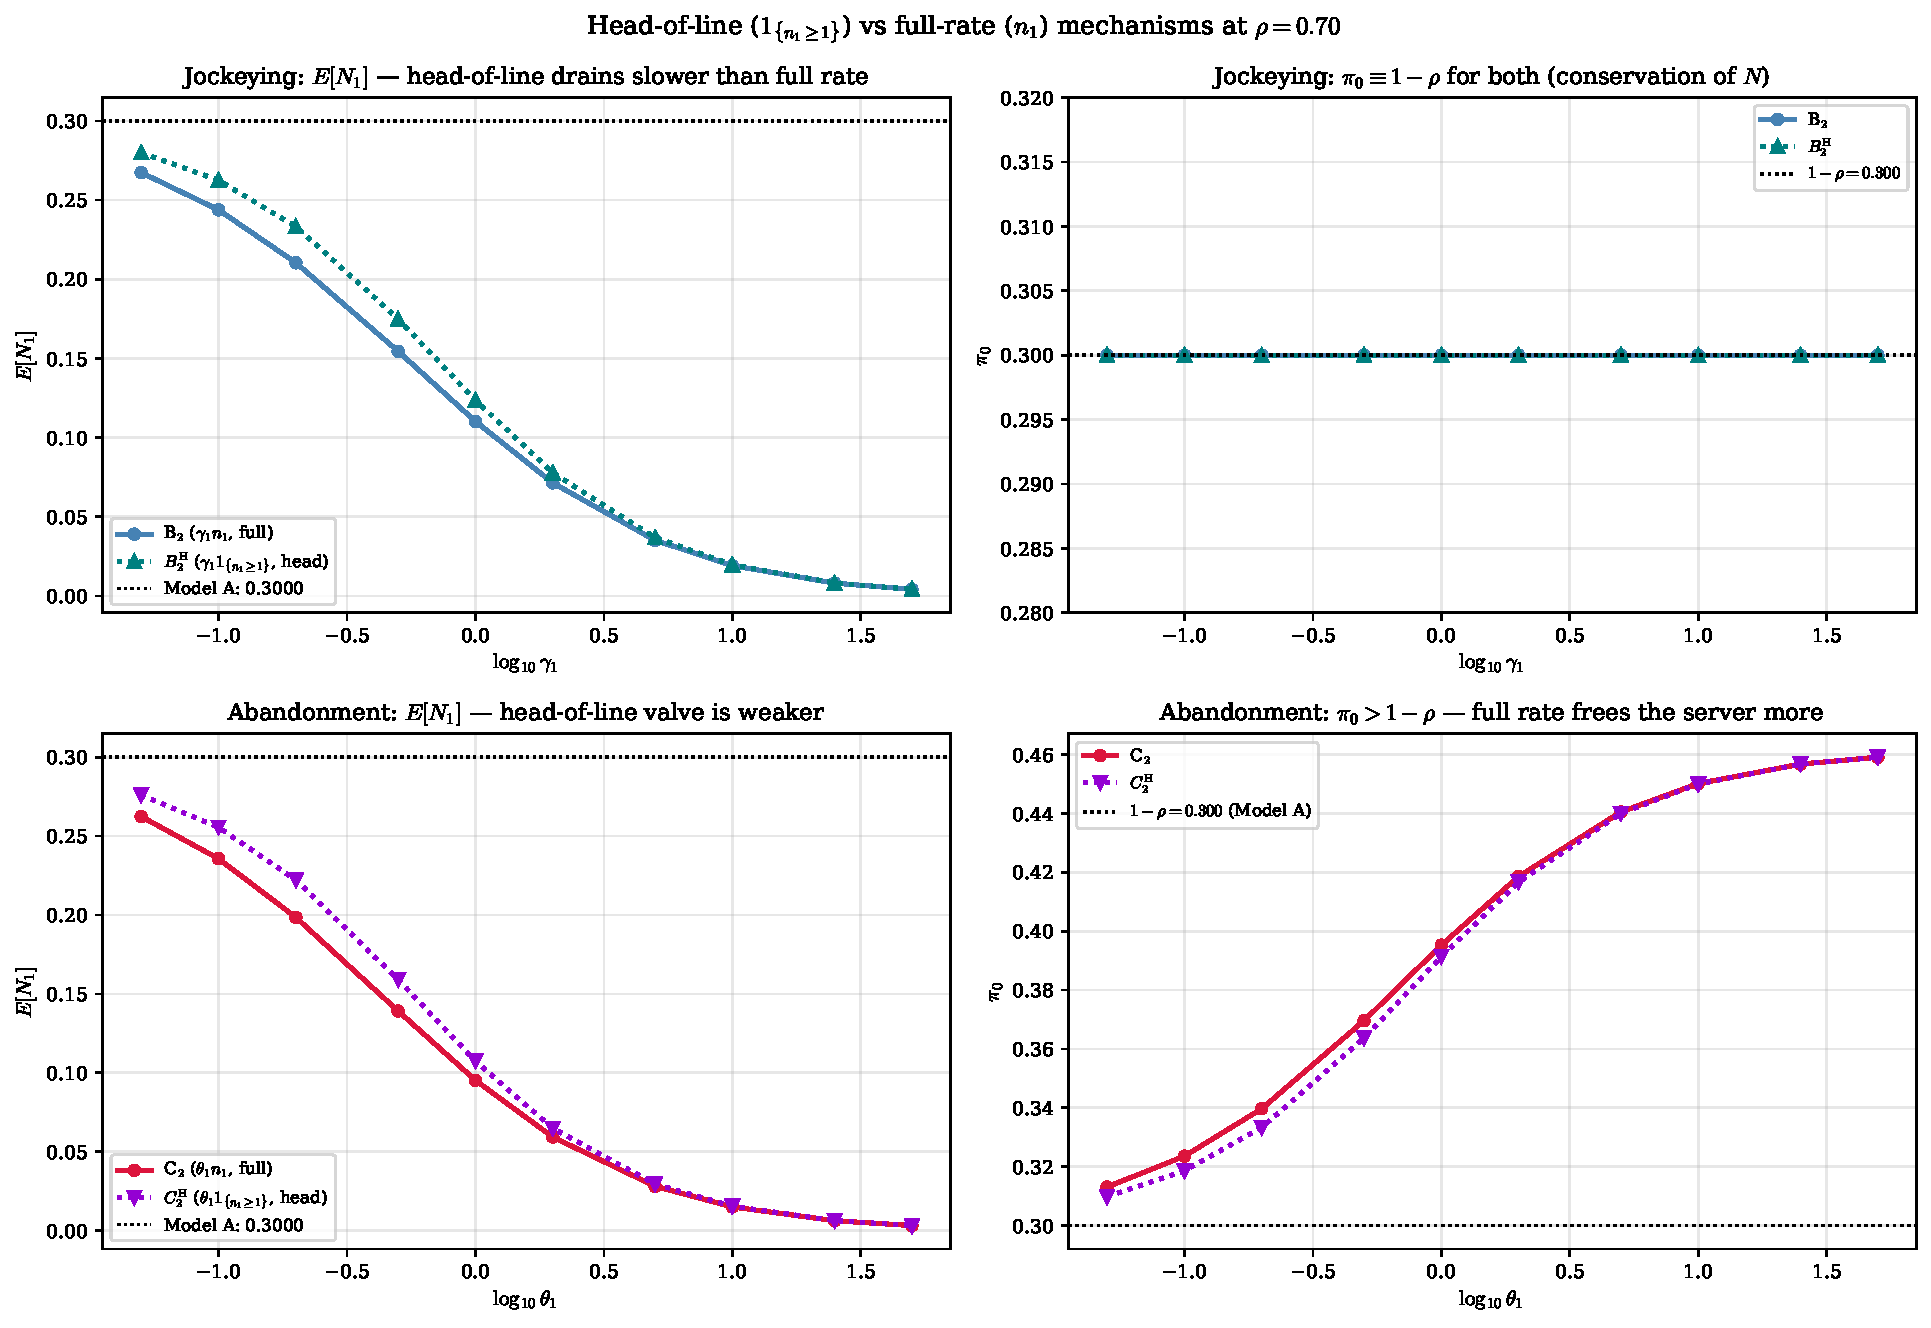
\includegraphics[width=0.98\textwidth]{figures/results/fig_hol_vs_full.pdf}
  \caption{Head-of-line ($\mathbf 1_{\{n_1\ge1\}}$) versus full-rate ($n_1$) mechanisms at
  $\rho=0.70$ ($\lambda_1=0.3$, $\lambda_2=0.4$, $\mu=1$). \emph{Top row, jockeying:}
  $\mathbb{E}[N_1]$ and $\pi_0$ for $B_2$ (full) versus $\BH$ (head-of-line). The
  head-of-line rate drains the priority queue more slowly, so $\mathbb{E}[N_1]$ stays above
  the $B_2$ curve, while $\pi_0\equiv1-\rho$ for both (jockeying conserves $N$,
  Corollaries~\ref{cor:B2:pi00}, \ref{cor:B21:pi0}). \emph{Bottom row, abandonment:}
  $\mathbb{E}[N_1]$ and $\pi_0$ for $C_2$ (full) versus $\CH$ (head-of-line). The
  head-of-line valve is weaker, so $\CH$ retains a slightly longer priority queue and a
  slightly smaller idle gain than $C_2$, both models exceeding the $1-\rho$ baseline
  (Corollaries~\ref{cor:C2:pi00}, \ref{cor:C21:pi0}).}
  \label{fig:comp:hol}
\end{figure}
%% END SIMULATION RESULTS — fig_hol_vs_full %%

The contrast is governed by the number of \emph{waiting} class-1 customers. When the
priority queue holds $n_1\ge2$, the full rate ejects customers at $n_1\gamma_1$ (or
$n_1\theta_1$), a factor of $n_1$ faster than the head-of-line rate $\gamma_1$ (or
$\theta_1$); when $n_1\le1$ the two rates coincide. The head-of-line model is therefore the
weaker drain precisely to the extent that $\mathbb{P}(N_1\ge2)$ carries mass, which is
greatest at intermediate mechanism rates and vanishes both as the rate $\to0$ (the queue is
rarely occupied beyond the head) and as the rate $\to\infty$ (the queue is emptied). The top
panels of Figure~\ref{fig:comp:hol} show this directly: at $\gamma_1=0.5$ the full rate cuts
$\mathbb{E}[N_1]$ from the Model-$A$ value $\ENoneASeventy$ to $\ENoneBtwoSeventy$ ($-\ENoneBtwoReductionSeventy\%$), whereas the
head-of-line rate reaches only $\ENoneBHSeventy$ ($-\ENoneBHReductionSeventy\%$); by $\gamma_1=50$ both have collapsed to
$\mathbb{E}[N_1]\approx0.004$ and the curves are indistinguishable.

This proxy can be read off the numbers directly. The full-versus-head-of-line gap in
$\mathbb{E}[N_1]$ grows with load --- $\gapENoneFifty$, $\gapENoneSeventy$, $\gapENoneNinety$
at $\rho=0.50,0.70,0.90$ --- and tracks the second-tail mass $\mathbb{P}(N_1\ge2)$, which over
the same loads is $\PNGetwoBtwoFifty$, $\PNGetwoBtwoSeventy$, $\PNGetwoBtwoNinety$ (Model-$B_2$).
The two move together because the full and head-of-line rates differ only on states with
$n_1\ge2$: where the priority queue seldom holds two or more waiting customers the cap costs
almost nothing, and where it often does the gap widens. The head-of-line $\mathbb{E}[N_1]$
excess is therefore an operational proxy for $\mathbb{P}(N_1\ge2)$, both vanishing at low load
and growing into the congested regime.

Because jockeying conserves the total customer count under either rate
(Corollary~\ref{cor:B21:pi0}), the milder class-1 drain of $\BH$ is mirrored by a milder
class-2 inflation: at $\rho=0.70$, $\mathbb{E}[N_2]=\ENtwoBHSeventy$ for $\BH$ against $\ENtwoBtwoSeventy$ for
$B_2$, and the priority ratio $\mathbb{E}[W_2]/\mathbb{E}[W_1]$ is $\premiumBHSeventy$ for $\BH$ versus
$\premiumBtwoSeventy$ for $B_2$ (Table~\ref{tab:comp:main}). Head-of-line jockeying thus erodes the
priority structure less aggressively than the full mechanism. The abandonment pair tells the
same story on the throughput--quality axis: at $\rho=0.70$ the full rate $C_2$ lifts $\pi_0$
to $\piZeroCtwoSeventy$ and compresses $\mathbb{E}[N]$ to $\ENCtwoSeventy$, while the head-of-line $\CH$ stops
at $\pi_0=\piZeroCHSeventy$ and $\mathbb{E}[N]=\ENCHSeventy$ --- it sheds less load, frees the server less,
and consequently leaves the priority ratio almost unchanged from the baseline
($\mathbb{E}[W_2]/\mathbb{E}[W_1]=\premiumCHSeventy$ for $\CH$ against $\premiumASeventy$ for $A$ and $\premiumCtwoSeventy$ for
$C_2$). In every descriptor the head-of-line variant interpolates monotonically between
Model-$A$ and its full-rate parent, confirming that restricting a mechanism to the head of
the queue yields a genuine but attenuated version of the same effect.

% =====================================================================
\subsection{Convergence to Model \texorpdfstring{$A$}{A}}
\label{app:numerics:convergence}

Every specialised model must recover Model-$A$ as its distinguishing parameter is switched
off. \S\ref{sec:comparison} established this algebraically and Section~\ref{sec:results}
reports the headline first-order rates; here the convergence is characterised figure by
figure, since the \emph{rate} of convergence measures how rapidly a mechanism departs from
the baseline as it is introduced. Convergence is measured in the $L_1$ distance
$\lVert\pi-\pi_A\rVert_1$ between the full joint distributions, supplemented by the
individual descriptors $\pi_0$, $\pi(0,0)$ and $\mathbb{E}[N_1]$.

\subsubsection{Model \texorpdfstring{$C_2$}{C2} as \texorpdfstring{$\theta_1\to0^+$}{theta1 to 0}}

%% BEGIN SIMULATION RESULTS — fig_conv_C2_to_A_L1 %%
\begin{figure}[H]
  \centering
  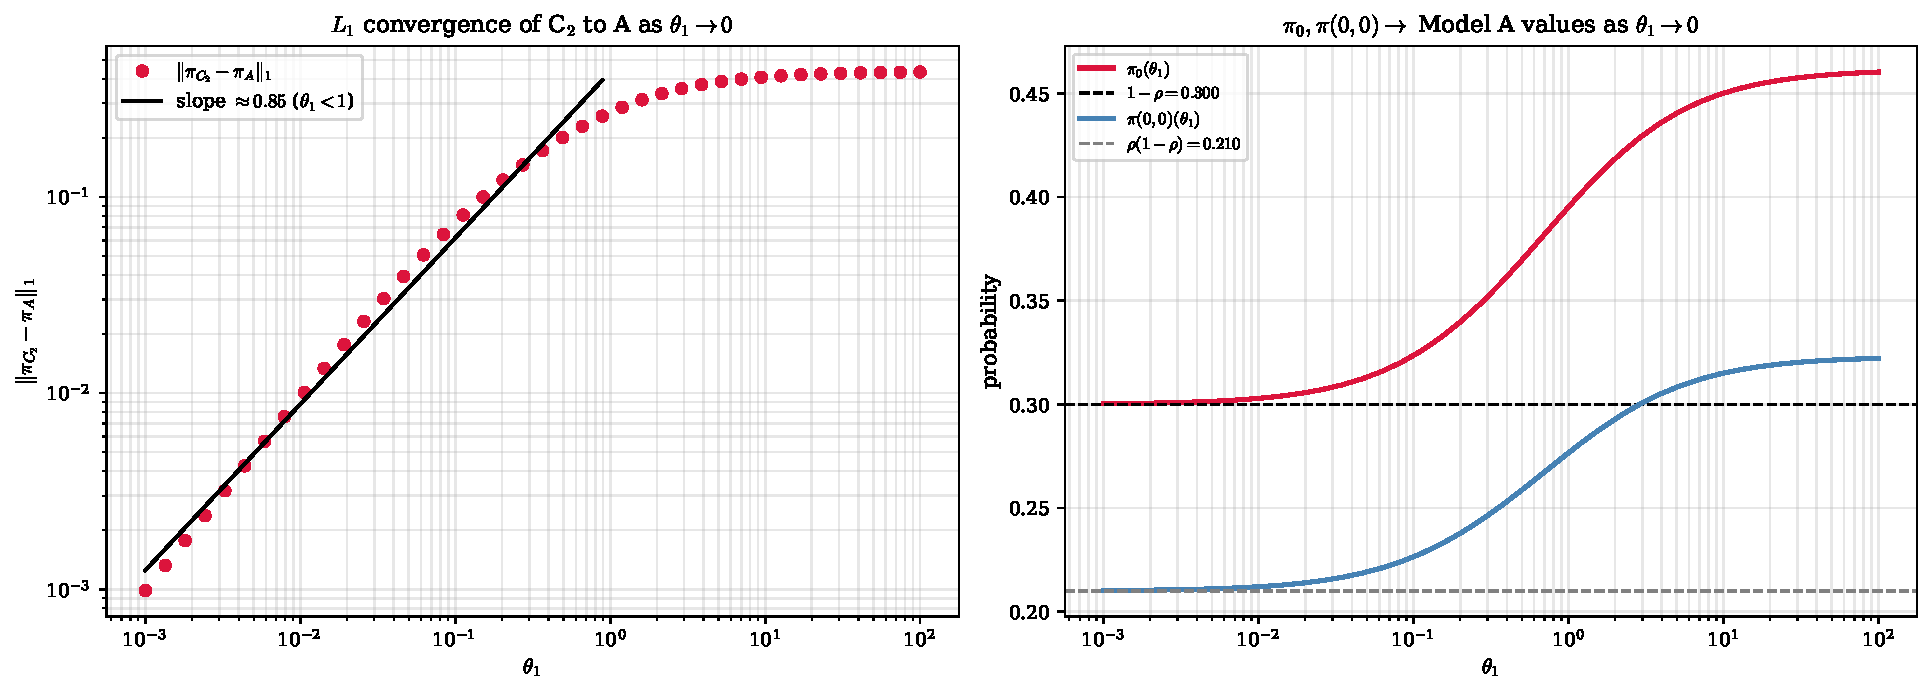
\includegraphics[width=0.98\textwidth]{figures/results/fig_conv_C2_to_A_L1.pdf}
  \caption{Convergence of Model-$C_2$ to Model-$A$ as $\theta_1\to0^+$
  ($\lambda_1=0.3$, $\lambda_2=0.4$, $\mu=1$). \emph{Left:} log--log plot of
  $\lVert\pi_{C_2}-\pi_A\rVert_1$ against $\theta_1$, with a fitted slope of $0.85$ over
  $\theta_1<1$. \emph{Right:} $\pi_0(\theta_1)$ and $\pi(0,0)(\theta_1)$ relaxing onto the
  Model-$A$ values $1-\rho=0.30$ and $\rho(1-\rho)=0.21$ as $\theta_1\to0$.}
  \label{fig:conv:c2_l1}
\end{figure}
%% END SIMULATION RESULTS — fig_conv_C2_to_A_L1 %%

%% BEGIN SIMULATION RESULTS — fig_conv_C2_to_A_indiv %%
\begin{figure}[H]
  \centering
  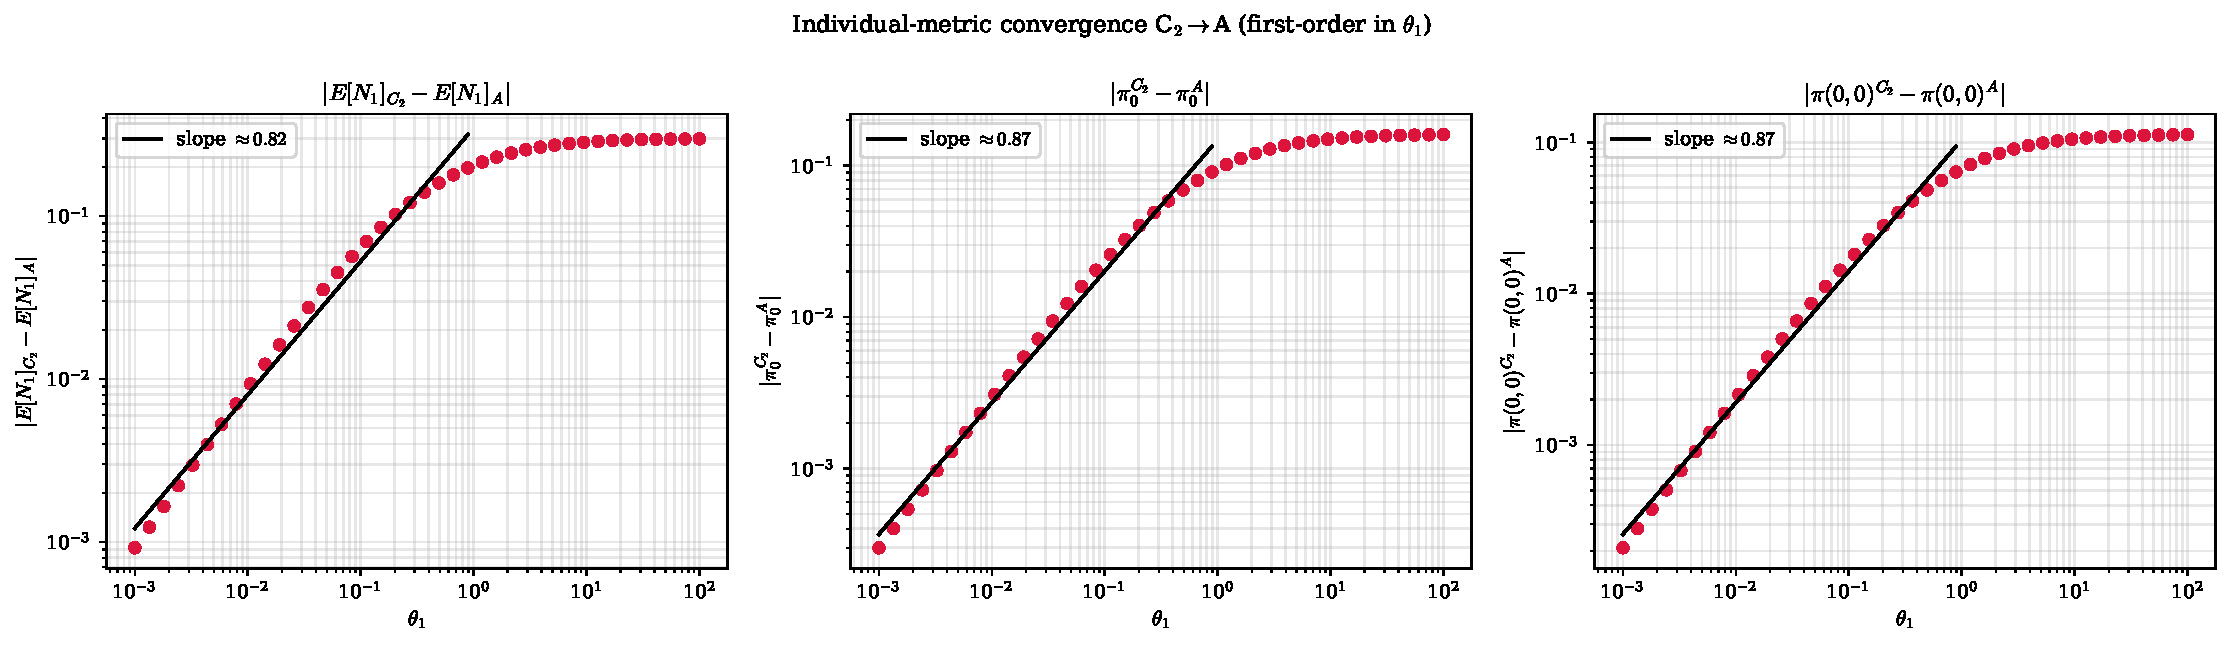
\includegraphics[width=0.98\textwidth]{figures/results/fig_conv_C2_to_A_indiv.pdf}
  \caption{Individual-descriptor convergence of $C_2\to A$: $|\mathbb{E}[N_1]_{C_2}-
  \mathbb{E}[N_1]_A|$, $|\pi_0^{C_2}-\pi_0^A|$ and $|\pi(0,0)^{C_2}-\pi(0,0)^A|$ versus
  $\theta_1$ on log--log axes, each annotated with its fitted slope.}
  \label{fig:conv:c2_indiv}
\end{figure}
%% END SIMULATION RESULTS — fig_conv_C2_to_A_indiv %%

Figure~\ref{fig:conv:c2_l1} examines the limit predicted by the
Corollary~\ref{cor:C2:pi00} statement that $\mathbb{E}[B_C]\to(\mu-\lambda_1)^{-1}$ as
$\theta_1\to0^+$, whence $\pi_0\to1-\rho$ and $\pi(0,0)\to\rho(1-\rho)$. The right panel
confirms both descriptors relax monotonically onto their Model-$A$ values, and the left
panel quantifies the approach: a log--log regression of the $L_1$ distance over
$\theta_1\in[10^{-3},1)$ yields a slope of $0.847$ (Table~\ref{tab:conv:rates}), consistent
with first-order convergence, $\lVert\pi_{C_2}-\pi_A\rVert_1=O(\theta_1)$. This matches the
analytic prediction: $\mathbb{E}[B_C]$ is smooth in $\theta_1$ at the origin, so its
first-order Taylor term governs the leading deviation. Figure~\ref{fig:conv:c2_indiv}
confirms that the individual descriptors converge at the same first-order rate
($\pi_0$ and $\pi(0,0)$ slopes both $0.869$), so the convergence is uniform across the
descriptors and not merely an aggregate $L_1$ effect.

\subsubsection{Model \texorpdfstring{$B_2$}{B2} as \texorpdfstring{$\gamma_1\to0^+$}{gamma1 to 0}}

%% BEGIN SIMULATION RESULTS — fig_conv_B2_to_A_L1 %%
\begin{figure}[H]
  \centering
  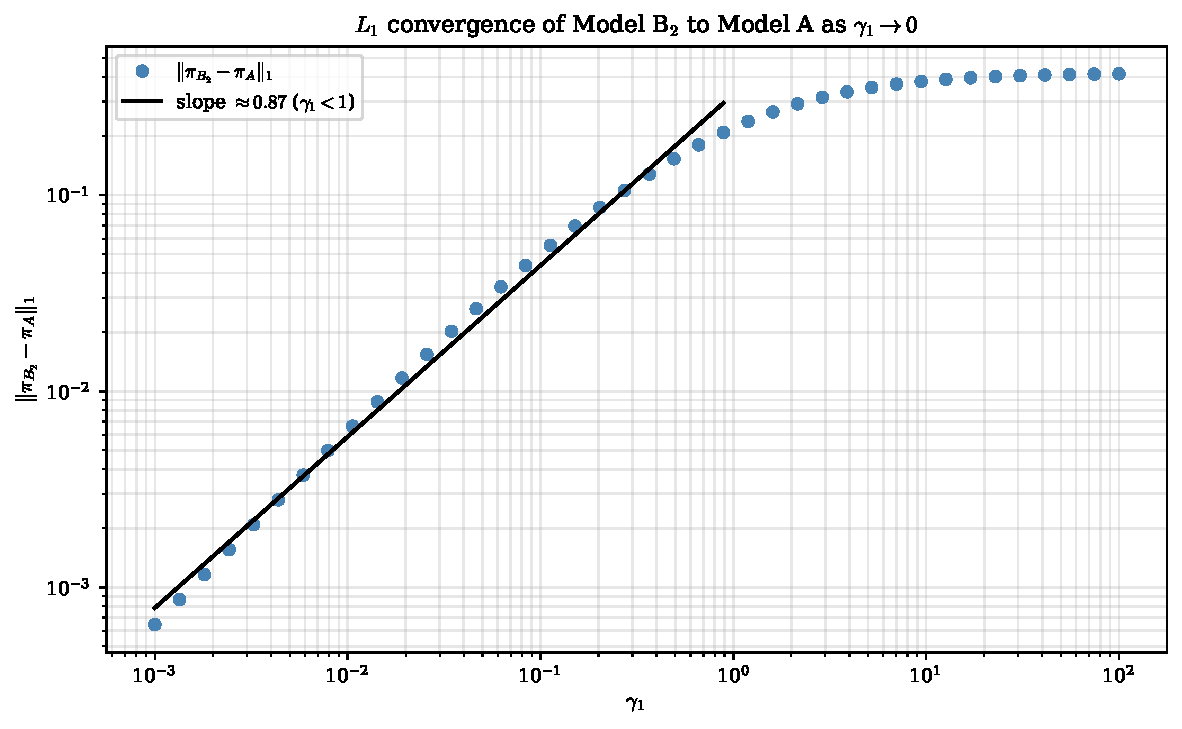
\includegraphics[width=0.78\textwidth]{figures/results/fig_conv_B2_to_A_L1.pdf}
  \caption{Convergence of Model-$B_2$ to Model-$A$ as $\gamma_1\to0^+$. The log--log $L_1$
  distance has fitted slope $0.87$ over $\gamma_1<1$, again first-order, even though the
  $B_2$ limit is singular in the ODE (the $\gamma_1\to0$ limit is non-uniform in the
  analytic continuation, but the stationary distribution responds at first order).}
  \label{fig:conv:b2_l1}
\end{figure}
%% END SIMULATION RESULTS — fig_conv_B2_to_A_L1 %%

For $B_2$ the limit is more delicate. As noted in \S\ref{sec:comparison}, $\gamma_1$
multiplies the highest-order term of the governing ODE, so $\gamma_1\to0$ is a singular
limit of the analytic solution. Nonetheless the \emph{stationary distribution} converges
smoothly: Figure~\ref{fig:conv:b2_l1} gives an $L_1$ slope of $0.873$
(Table~\ref{tab:conv:rates}), first-order in $\gamma_1$. The descriptors $\pi_0$ and
$\pi(0,0)$ require no convergence analysis at all --- by Corollary~\ref{cor:B2:pi00} they
equal their Model-$A$ values \emph{identically} for every $\gamma_1>0$, so their deviation
sits at the numerical floor and the corresponding entries in Table~\ref{tab:conv:rates} are
not meaningful. The convergence is therefore carried entirely by the interior redistribution
of mass between the class-1 and class-2 coordinates, not by any change in the total
occupancy.

\subsubsection{Instant-jockeying limit \texorpdfstring{$\gamma_1\to\infty$}{gamma1 to infinity}}

%% BEGIN SIMULATION RESULTS — fig_conv_B2_inf_jockeying %%
\begin{figure}[H]
  \centering
  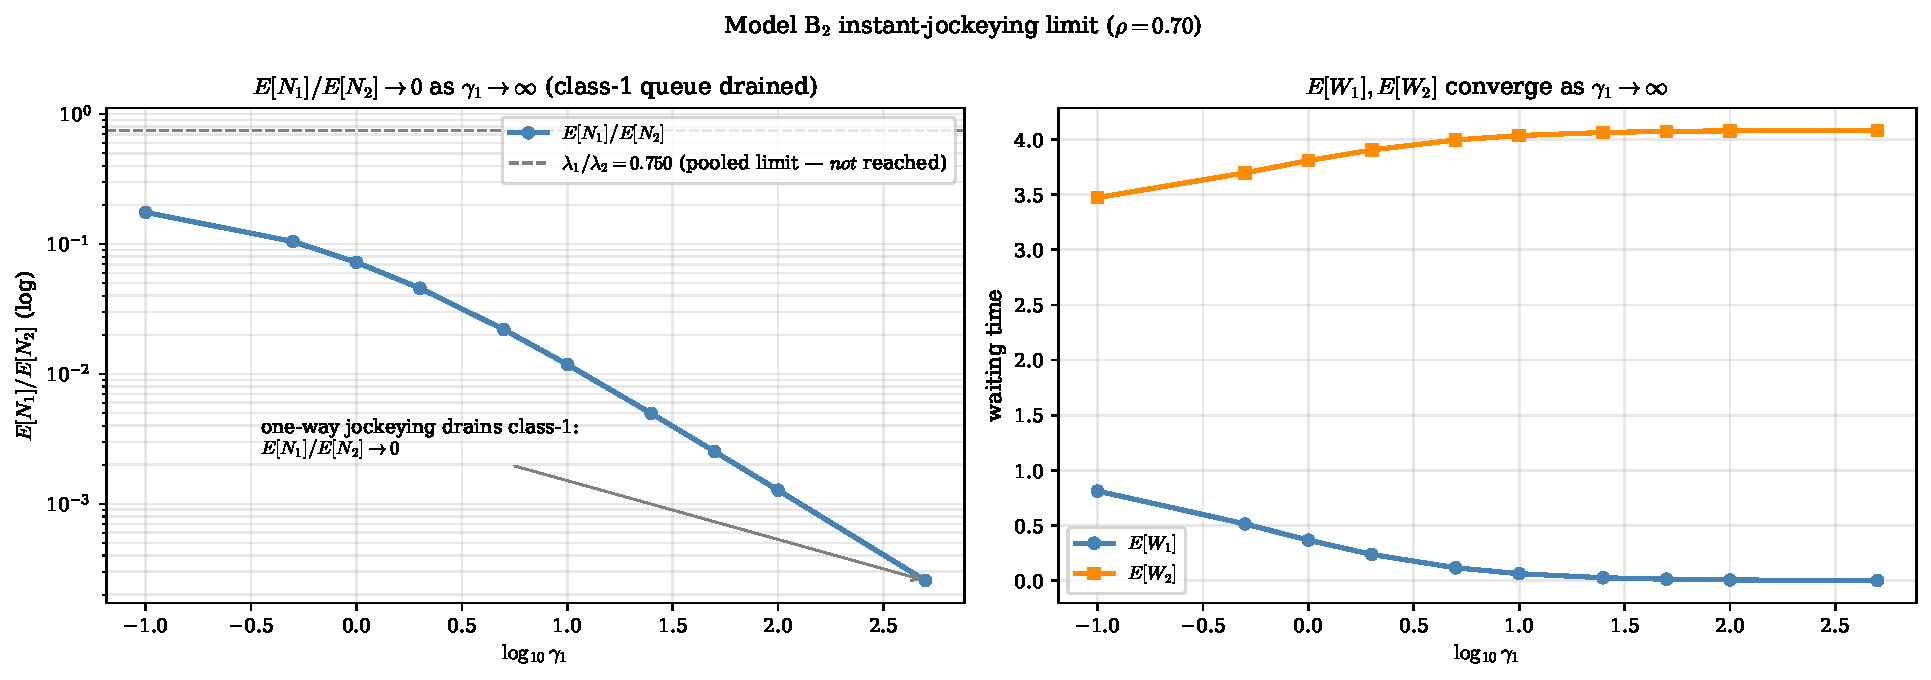
\includegraphics[width=0.98\textwidth]{figures/results/fig_conv_B2_inf_jockeying.pdf}
  \caption{Model-$B_2$ in the strong-jockeying regime $\gamma_1\to\infty$ at $\rho=0.70$.
  \emph{Left:} $\mathbb{E}[N_1]/\mathbb{E}[N_2]\to0$ (note the logarithmic ordinate): one-way
  jockeying is absorbing, so the class-1 queue is drained completely. \emph{Right:}
  $\mathbb{E}[W_1]\to0$ while $\mathbb{E}[W_2]$ saturates as $\mathbb{E}[N_2]\to\mathbb{E}[N]_A$.}
  \label{fig:conv:b2_inf}
\end{figure}
%% END SIMULATION RESULTS — fig_conv_B2_inf_jockeying %%

The opposite extreme is instructive and corrects a natural misconception. One might expect
the strong-jockeying limit to balance the two queues in proportion to their arrival rates,
$\mathbb{E}[N_1]/\mathbb{E}[N_2]\to\lambda_1/\lambda_2$, as a two-way exchange would. But the
$B_2$ jockeying is \emph{one-way} ($1\!\to\!2$): it has no return channel, so it is
absorbing into class~2. As $\gamma_1\to\infty$ every class-1 arrival is converted on
essentially zero timescale and the class-1 queue is drained,
$\mathbb{E}[N_1]/\mathbb{E}[N_2]\to0$ --- the computed ratio
(Figure~\ref{fig:conv:b2_inf}, left) falls from $0.1045$ at
$\gamma_1=0.5$ to $3\times10^{-4}$ at $\gamma_1=500$, with no sign of levelling at
$\lambda_1/\lambda_2=0.75$. Because jockeying conserves $N$, the entire occupancy migrates
to class~2, $\mathbb{E}[N_2]\to\mathbb{E}[N]_A=\ENASeventy$, and correspondingly
$\mathbb{E}[W_1]\to0$ while $\mathbb{E}[W_2]$ saturates. The limit confirms that one-way
jockeying does not pool the system but rather extinguishes the priority class as a distinct
queue.

\subsubsection{Head-of-line models \texorpdfstring{$\BH$}{B2-H} and \texorpdfstring{$\CH$}{C2-H}}

The two head-of-line experiment models must also recover Model-$A$ as their mechanism
parameter is switched off: as $\gamma_1\to0^+$ (Model-$\BH$) or $\theta_1\to0^+$
(Model-$\CH$) the kernel quadratic loses its $\gamma_1$/$\theta_1$ shift and the rational
PGF of Theorems~\ref{thm:B21:PGF} and~\ref{thm:C21:PGF} collapses to the Model-$A$ form of
Theorem~\ref{thm:A:PGF}. Figure~\ref{fig:conv:experiment} verifies both limits numerically.

%% BEGIN SIMULATION RESULTS — fig_conv_experiment_to_A %%
\begin{figure}[H]
  \centering
  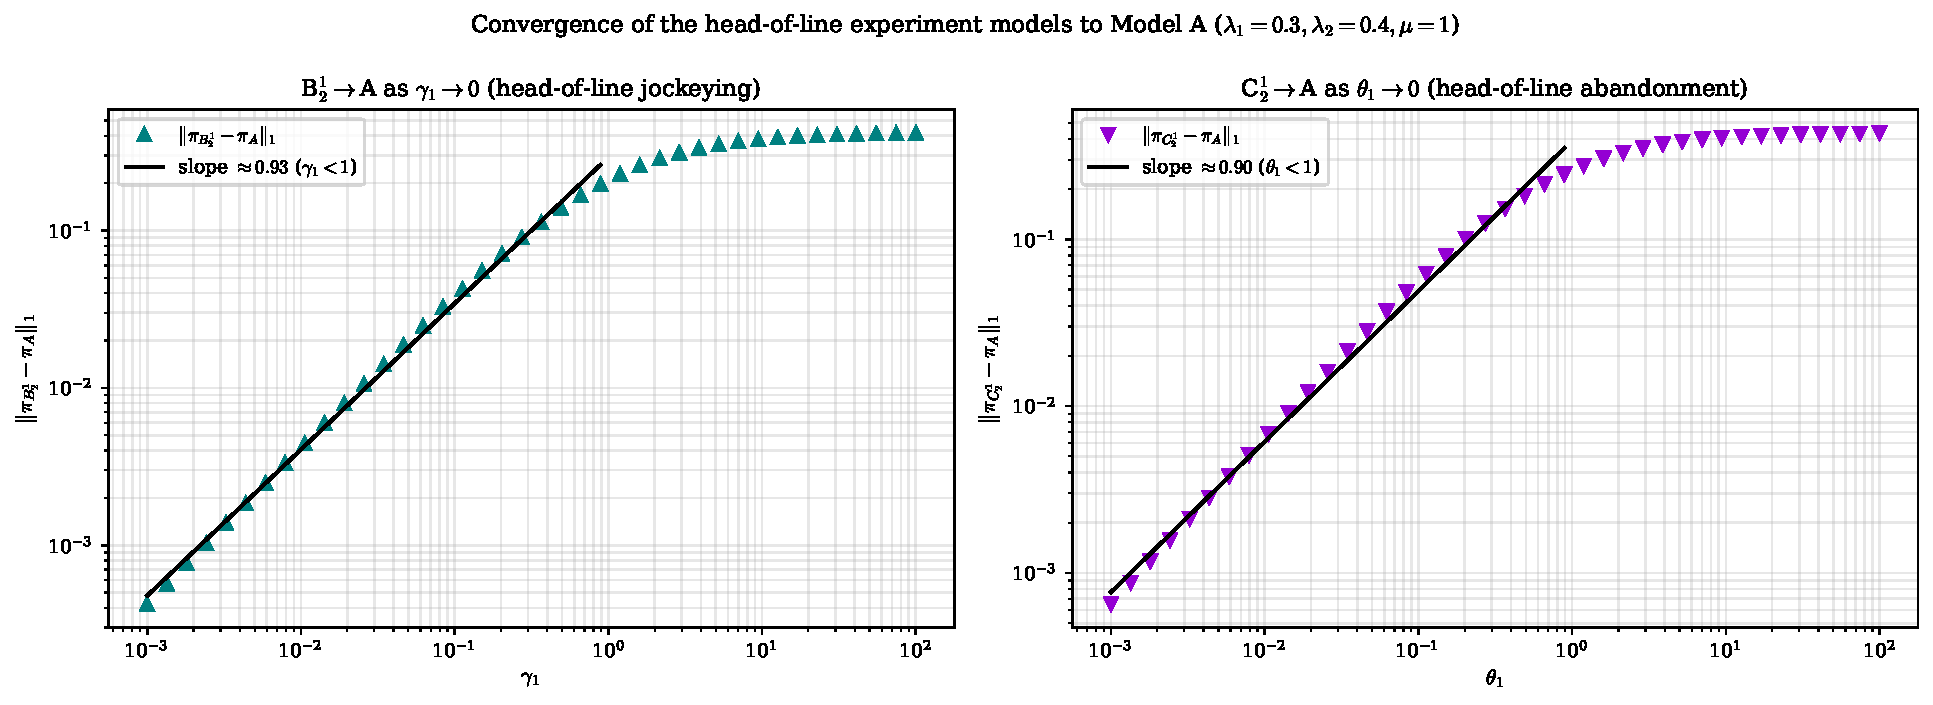
\includegraphics[width=0.98\textwidth]{figures/results/fig_conv_experiment_to_A.pdf}
  \caption{Convergence of the head-of-line experiment models to Model-$A$
  ($\lambda_1=0.3$, $\lambda_2=0.4$, $\mu=1$). \emph{Left:} log--log plot of
  $\lVert\pi_{\BH}-\pi_A\rVert_1$ against $\gamma_1$, with the fitted first-order slope.
  \emph{Right:} $\lVert\pi_{\CH}-\pi_A\rVert_1$ against $\theta_1$, likewise first-order.
  Both head-of-line variants approach the baseline at the same order as their full-rate
  counterparts $B_2$ and $C_2$.}
  \label{fig:conv:experiment}
\end{figure}
%% END SIMULATION RESULTS — fig_conv_experiment_to_A %%

The mechanism is the analytic counterpart of the full-rate case: because both
$\gamma_1\mathbf{1}_{\{n_1\ge1\}}$ and $\theta_1\mathbf{1}_{\{n_1\ge1\}}$ enter the
fundamental equation linearly in the mechanism parameter, the stationary distribution is
smooth at the origin and its first-order Taylor term governs the leading deviation. For
$\BH$ the conserved descriptors $\pi_0$ and $\pi(0,0)$ equal their Model-$A$ values
identically for every $\gamma_1>0$ (Corollary~\ref{cor:B21:pi0}), exactly as for $B_2$, so
the $L_1$ approach is again carried entirely by the interior redistribution of mass between
the two coordinates; for $\CH$ the descriptors $\pi_0$ and $\pi(0,0)$ relax onto the
baseline at the same first order, since the closed forms~\eqref{eq:C21:pi0_pi00} are smooth
in $\theta_1$ at zero.

%% BEGIN SIMULATION RESULTS — tab_convergence_rates %%
\begin{table}[t]\centering
\caption{Empirical convergence rates of Models C$_2$ and B$_2$ to Model A, from log-log regression of the deviation against the mechanism parameter (fit over parameter $<1$).}
\label{tab:conv:rates}
\begin{tabular}{llrrrl}
\toprule
Limit & Parameter & $L_1$ slope & $\pi_0$ slope & $\pi(0,0)$ slope & Valid range \\
\midrule
C$_2\to$A & $\theta_1\to0$ & 0.847 & 0.869 & 0.869 & $\theta_1\in[10^{-3},1)$ \\
B$_2\to$A & $\gamma_1\to0$ & 0.873 & 0.348 & 0.211 & $\gamma_1\in[10^{-3},1)$ \\
\bottomrule
\end{tabular}
\footnotesize\par\vspace{2pt}For B$_2$, $\pi_0$ and $\pi(0,0)$ are $\gamma_1$-invariant (jockeying conserves $N$), so their deviations are at the numerical floor and the slope is not meaningful (n/a).
\end{table}

%% END SIMULATION RESULTS — tab_convergence_rates %%

Table~\ref{tab:conv:rates} collects the empirical convergence rates for all four specialised
models. Each approaches Model-$A$ at first order in its distinguishing parameter --- $L_1$
slopes of $0.847$ ($C_2$), $0.903$ ($\CH$), $0.873$ ($B_2$) and $0.929$
($\BH$), each within the $0.1$--$0.2$ tolerance band of the theoretical exponent $1$. The
slight shortfall below unity is a finite-truncation and finite-grid artefact of the
log--log fit, not a genuine fractional rate, and requires no further investigation. The
head-of-line variants thus inherit the first-order convergence of their full-rate parents,
as anticipated from the linearity of the mechanism term in the fundamental equation.

% =====================================================================
\subsection{Comparative dashboard}
\label{subsec:results:dashboard}

%% BEGIN SIMULATION RESULTS — fig_summary_dashboard %%
\begin{figure}[H]
  \centering
  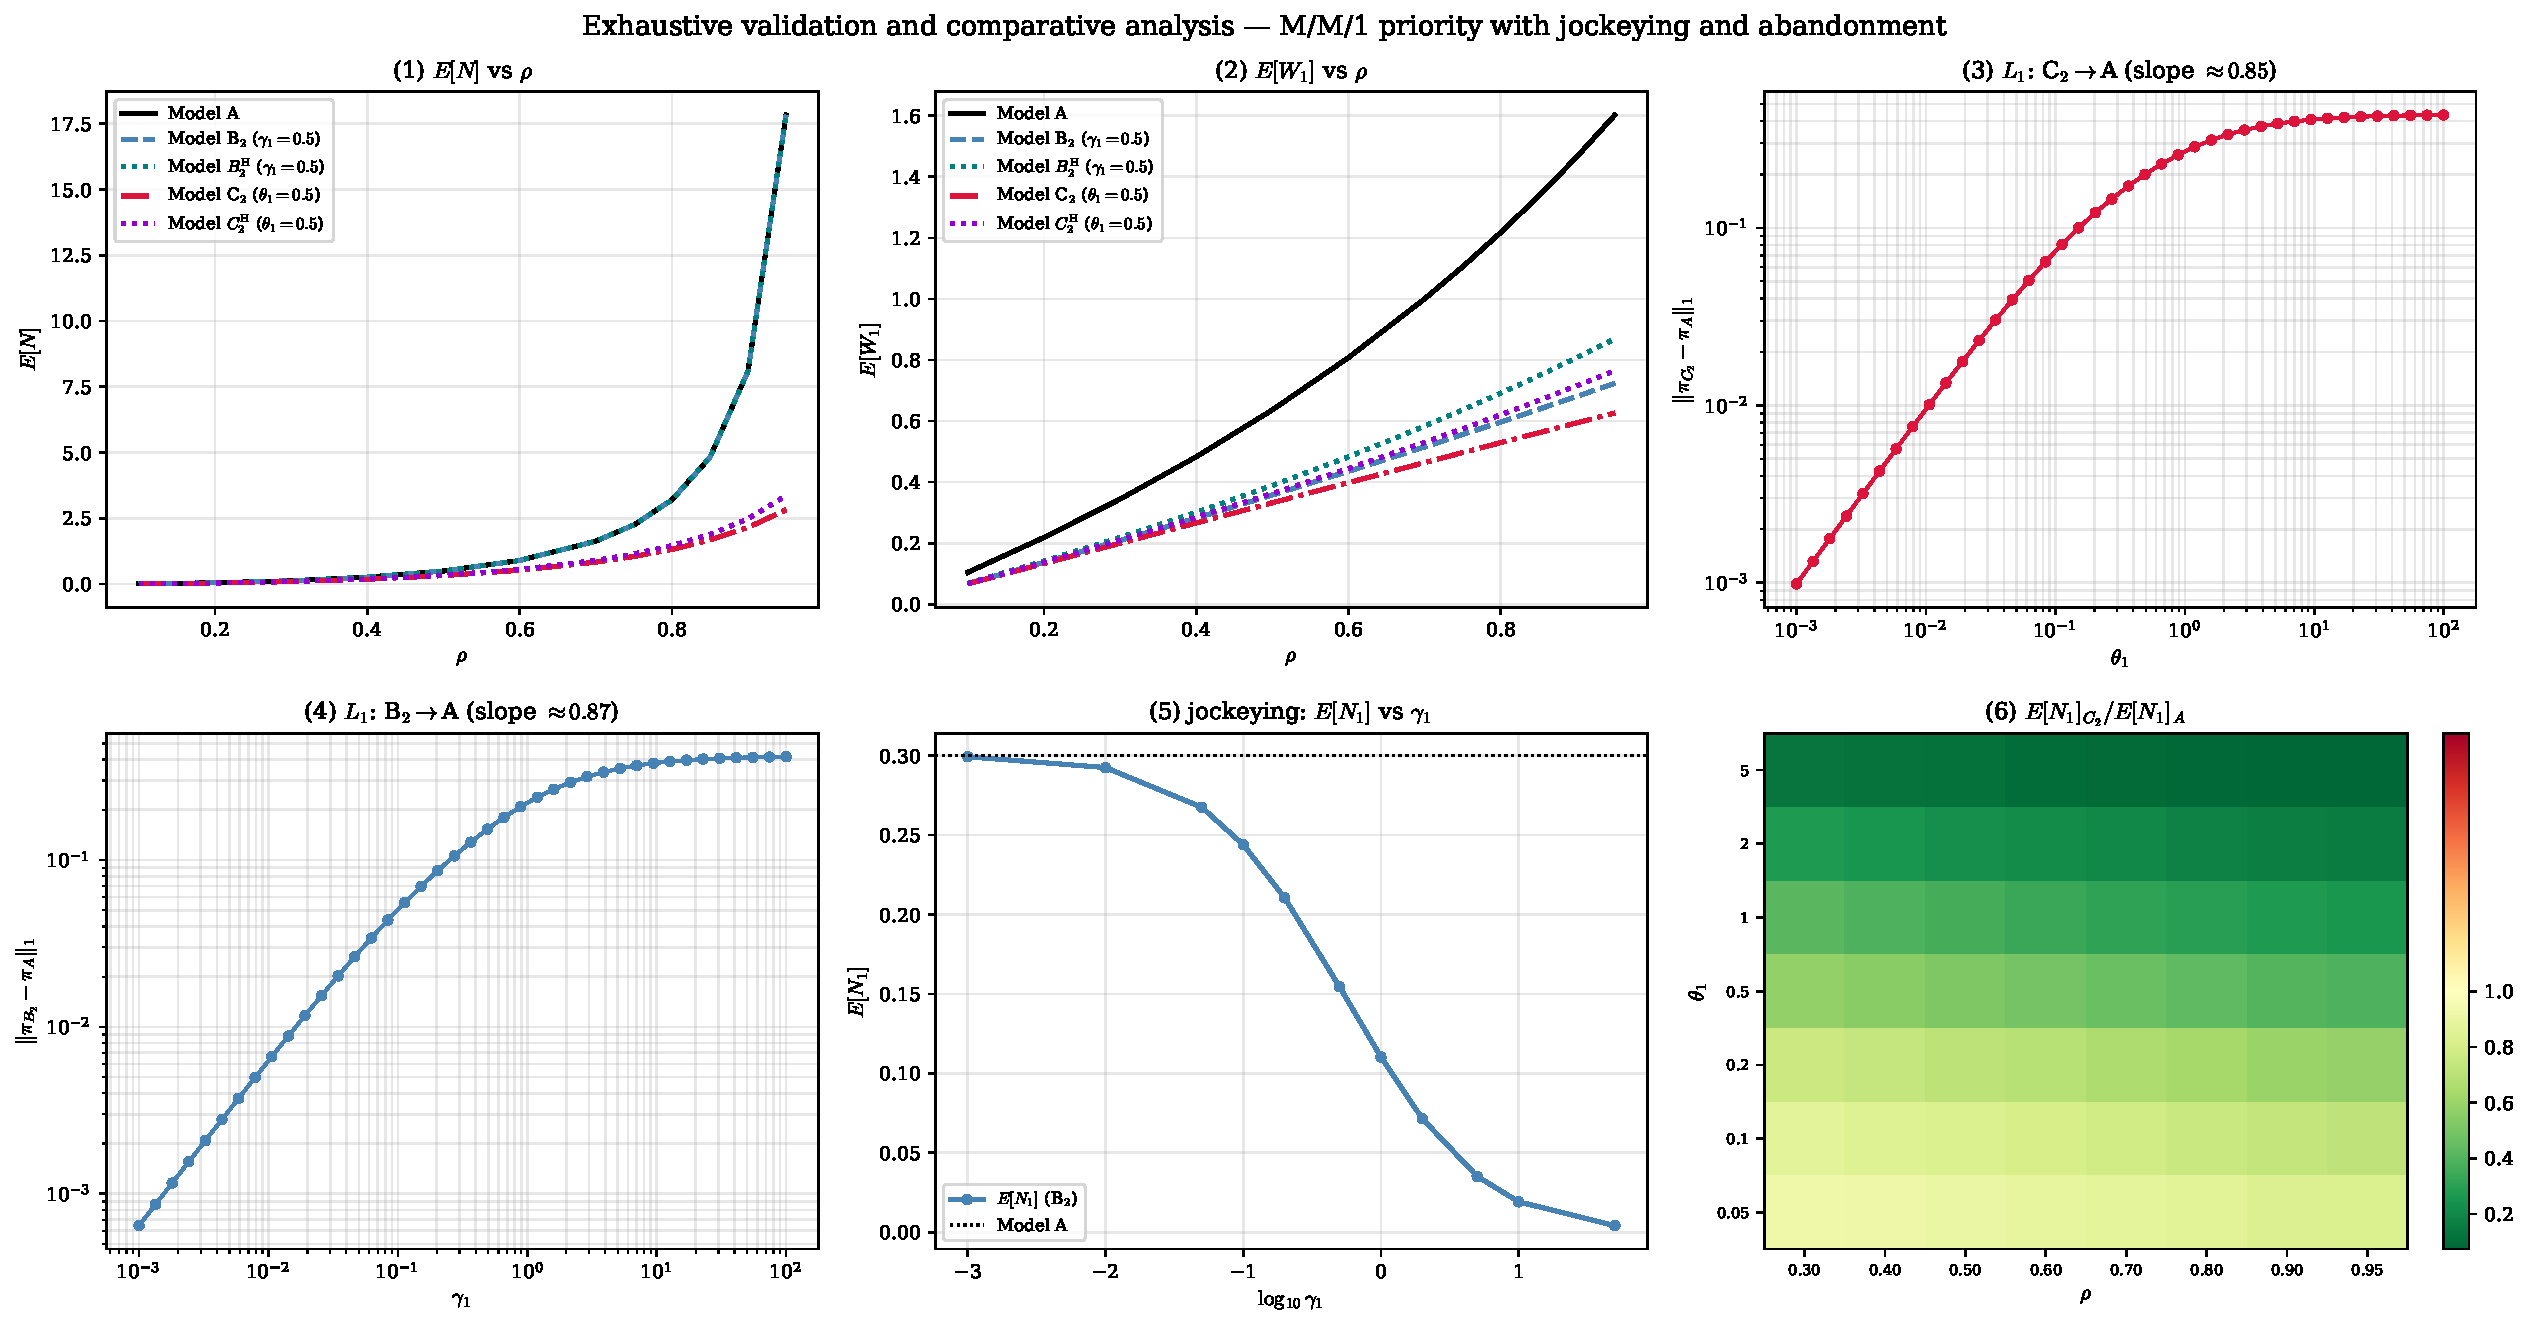
\includegraphics[width=\textwidth]{figures/results/fig_summary_dashboard.pdf}
  \caption{Synoptic dashboard of the numerical study: (1)~$\mathbb{E}[N]$ and
  (2)~$\mathbb{E}[W_1]$ versus $\rho$ for all five solved models (A, $B_2$, $\BH$, $C_2$,
  $\CH$); (3)~$L_1$ convergence $C_2\to A$ and
  (4)~$B_2\to A$; (5)~the jockeying effect on $\mathbb{E}[N_1]$; and (6)~the
  $\mathbb{E}[N_1]_{C_2}/\mathbb{E}[N_1]_A$ heatmap over $(\rho,\theta_1)$. Together these
  panels summarise the two central findings: jockeying redistributes delay at fixed total
  work, while abandonment reduces total work at a throughput cost.}
  \label{fig:results:dashboard}
\end{figure}
%% END SIMULATION RESULTS — fig_summary_dashboard %%

Figure~\ref{fig:results:dashboard} assembles the six most informative panels of the study in
a single view. It restates at a glance the contrast developed analytically in
\S\ref{sec:comparison}: the $A$ and $B_2$ load curves coincide while $C_2$ sits below them,
the two convergence panels exhibit the common first-order approach to the baseline, and the
heatmap localises the regime in which abandonment is most effective as a congestion control.
